\documentclass[
    iai, % Saisir le nom de l'institut rattaché
    eai, % Saisir le nom de l'orientation
    %confidential, % Décommentez si le travail est confidentiel
]{heig-tb}

\usepackage[nooldvoltagedirection,european,americaninductors]{circuitikz}

\signature{mbernasconi.svg} % Remplacer par votre propre signature vectorielle.

\makenomenclature
\makenoidxglossaries
\makeindex

\addbibresource{bibliography.bib}

\input{nomenclature}
\newacronym{gcd}{GCD}{Plus grand diviseur commun}
\newacronym{lcm}{LCM}{Plus petit multiple commun}
\newacronym{rpi4}{Rpi4}{Rapsberry Pi 4b}

\newglossaryentry{heig-vd}{
    name=HEIG-VD,
    description={Haute École d'Ingénierie et de Gestion du canton de Vaud}
}
\newglossaryentry{hes-so}{
    name=HES-SO,
    description={Haute École Supérieure de Suisse Occidentale}
}
\newglossaryentry{latex}{
    name=latex,
    description={Un langage et un système de composition de documents}
}
\newglossaryentry{maths}{
    name=mathematics,
    description={Les mathematiques sont ce que les mathématiciens fonts}
}

\newglossaryentry{mir}{
    name=MIR,
    description={Infrarouge moyen}
}

\newglossaryentry{ir}{
    name=IR,
    description={Infrarouge}
}

\newglossaryentry{iso}{
    name=ISO,
    description={Organisation internationale de normalisation}
}

\newglossaryentry{wifi}{
    name=WiFi,
    description={wireless fidelity}
}

\newglossaryentry{fps}{
    name=FPS,
    description={frame per seconde}
}

\newglossaryentry{chf}{
    name=CHF,
    description={Confoederatio Helvetica Franc - Franc Suisse}
}

\newglossaryentry{fablab}{
    name=FabLab,
    description={Atelier de fabrication de l'HEIG-VD - salle C08}
}

\newglossaryentry{reds}{
    name=ReDS,
    description={Institut de recherche appliquée et développement de la HEIG-VD}
}

\newglossaryentry{rpi4}{
    name=Rpi4,
    description={Rapsberry Pi 4}
}
% Auteur du document (étudiant-e) en projet de Bachelor
\author{Adriano Vieux}

% Activer l'option pour l'accord du féminin dans le texte
\genre{male}

% Titre de votre travail de Bachelor
\title{Détection de traces d'hydrocarbures sur route par vision industrielle}

% Le sous titre est optionnel
\subtitle{Travail de Bachelor}

% Nom du professeur responsable
\teacher {Prof. P. Bressy (HEIG-VD)}

% Mettre à jour avec la date de rendu du travail
\date{\today}

% Numéro de TB
\thesis{7333}


\surroundwithmdframed{minted}

%% Début du document
\begin{document}
\selectlanguage{french}
\maketitle
\frontmatter
\clearemptydoublepage

%% Requis par les dispositions générales des travaux de Bachelor
\preamble
\authentification

%% Résumé / Résumé publiable / Version abrégée
\begin{abstract}
    % Francais
Le but de ce travail de Bachelor est de mettre en place un système permettant détecter et agir sur les hydrocarbures aux sols par vision industrielle. Actuellement, lorsque les pompiers interviennent pour des cas de fuites d'hydrocarbures sur routes, ils utilisent une remorque-semeuse qu'ils contrôle manuellement afin de déverser du produit absorbant sur les zones à traiter.

La détection est basée sur un éclairage infrarouge et d'un capteur adapté transmettant les captures de la zone à observer vers un boitier de traitement. L'analyse de l'image permet de définir les zones sur lesquelles agir. Un algorithme détermine ensuite où verser le produit absorbant en fonction des données reçues et de la vitesse du véhicule.


\asterism

% English
The purpose of this Bachelor's thesis is to develop a system that can detect and respond to hydrocarbons on the ground using industrial vision. Currently, when firefighters respond to cases of hydrocarbon leaks on roads, they use a manually controlled spreading trailer to spread absorbent material on the affected areas.

The detection is based on infrared illumination and a suitable sensor that transmits captured images of the observed area to a processing unit. The image analysis allows for identifying the areas that need treatment. An algorithm then determines where to apply the absorbent material based on the received data and the vehicle speed.


\end{abstract}

%% Sommaire et tables
\clearemptydoublepage
{
    \tableofcontents
    \let\cleardoublepage\clearpage
    \listoffigures
    \let\cleardoublepage\clearpage
    \listoftables
    \let\cleardoublepage\clearpage
    \listoflistings
}

\printnomenclature
\clearemptydoublepage
\pagenumbering{arabic}

%% Contenu
\mainmatter
\chapter{Introduction}
\section{Contexte}
En l'état actuel, lorsque les pompiers doivent intervenir dans le cas d'un incident impliquant des fuites d'hydrocarbures sur route, la répartition
du produit absorbant se fait via une remorque-semoirs. Celle-ci dispose de trois sections de dépose de produit qui sont télécommandées directement par un opérateur.
Durant l'intervention, une personne doit marcher à côté de la remorque afin d'observer et contrôler la répartition du produit, nous pouvons relever les points suivant:
\begin{enumerate}
    \item L'opérateur doit marcher, cela limite la vitesse du véhicule et les longues distances sont problématiques.
    \item La détection se fait à l'oeil nu, l'opérateur doit donc rester concentrer en permanence au risque de devoir repasser sur certaines zone.
    \item La commande est manuelle, il est possible de faire des erreurs sur la commande risquant la dépose de surplus de produit ou de devoir repasser sur certaines zone.
\end{enumerate}
\textbf{Le but de se travail de Bachelor est d'automatiser ce processus, via un système de détection des hydrocarbures par vision industrielle et d'un pilotage de l'ouverture/fermeture des vérins.}
\section{Cahier des charges \label{cdc}}
Le cahier des charges est le suivant:
\begin{itemize}
    \item Préparer un planning détaillant les tâches.
    \item Définir un setup permettant de:
          \begin{itemize}
              \item Analyser les traces d'hydrocarbures selon leur positionnement sur la route.
              \item Commander la télécommande du semoir.
          \end{itemize}
    \item Sélectionner les éléments composant le setup.
    \item Commander les éléments.
    \item Assembler les éléments.
    \item Tester le setup et procéder aux ajustements nécessaires.
    \item Développer un logiciel d'analyse et de gestion de la télécommande.
    \item Tester le logiciel d'analyse et de gestion de la télécommande.
    \item Valider le logiciel et le comportement sur la route.
    \item Analyser et interpréter les résultats.
\end{itemize}
\section{Planning}
Le planning vient compléter le cahier des charges du chapitre \ref{cdc} en ajoutant le travail à effectuer pour chaque étape ainsi qu'une estimation
de l'effort à fournir en heure.

Le planning ci-dessous présente les étapes, le détail des sous-étapes, l'effort à fournir estimé ainsi que la période durant laquelle chaque étape sera présumément effectuée (en bleu).
\begin{figure}[H]
    \centering
    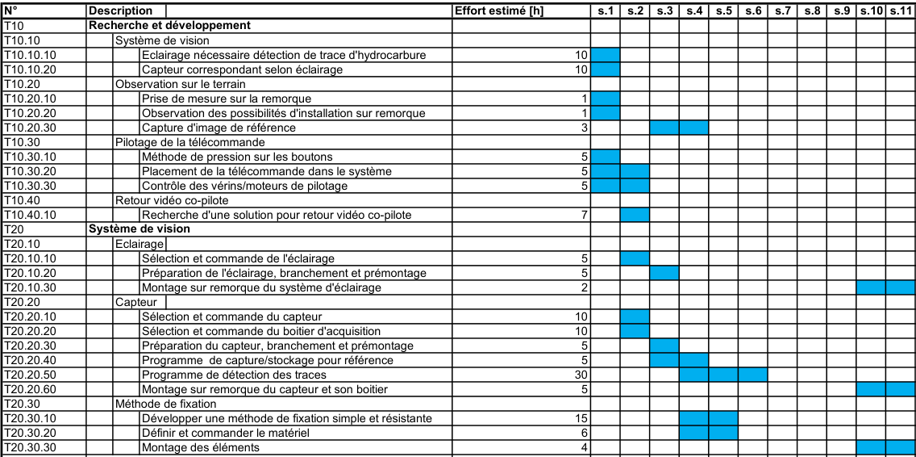
\includegraphics[width=15cm, angle=90]{assets/figures/planning1.png}
    \caption{Planning - partie 1}
\end{figure}
\newpage
\begin{figure}[H]
    \centering
    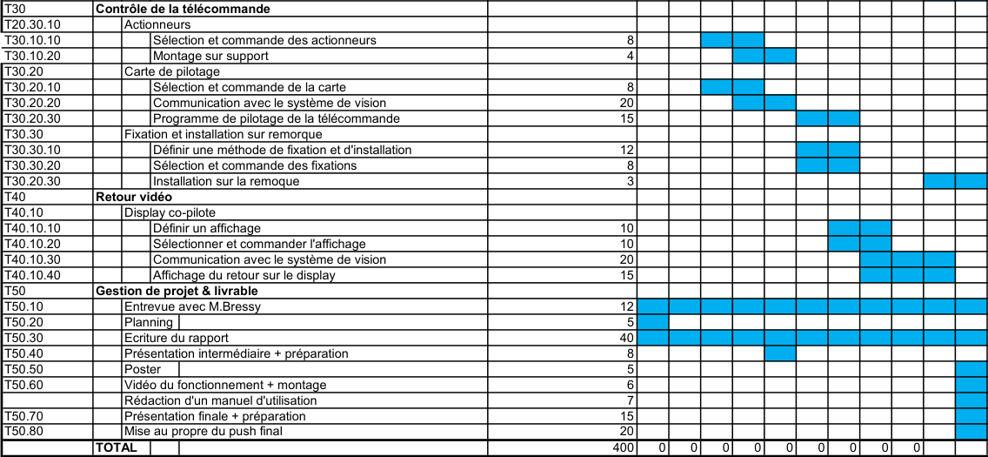
\includegraphics[width=15cm, angle=90]{assets/figures/planning2.png}
    \caption{Planning - partie 2}
\end{figure}

En complément au planning ci-dessus, on peut imaginer une vingtaine d'heures d'imprévus supplémentaires.
%%if
\section{Exemple d'équation}
L'une des principales forces de \LaTeX~est la saisie d'équations. L'équation \ref{eq:1}, citée à titre d'exemple, représente la transformation de phase d'une lentille biconvexe. Pour rédiger une équation \LaTeX~vous pouvez utiliser des outils en ligne tels que \href{https://www.latex4technics.com/}{latex4technics}. Essayez autant que possible d'écrire vos équations à la main. La courbe d'apprentissage n'est pas très raide et la valeur ajoutée est grande. Vous pouvez vous aider du panneau de \LaTeX~Workshop dans Visual Studio Code. Il est accessible via le raccourcis clavier \keystroke{Ctrl} + \keystroke{Alt} + \keystroke{X}.

\begin{equation} \label{eq:1}
    \begin{split}
        L(x,y) &= \exp\left( - i\frac{{2\pi }}{\lambda }\left( {n\Delta \varphi (x,y) + \Delta {\varphi _0} - \Delta \varphi (x,y)} \right)\right)\\
        &= {\exp\left({i\frac{{2\pi }}{\lambda }\Delta {\varphi _0}}\right)}{\exp\left({ - i\frac{{2\pi }}{{\lambda f}}({x^2} + {y^2})}\right)}
    \end{split}
\end{equation}

\section{Exemples de diagrammes}

Les diagrammes de flux peuvent être réalisés en utilisant l'outil \href{https://app.diagrams.net/}{draw.io}. Une exportation en \texttt{.drawio} (non compressé) permet de garder les sources de la figure. Le rendu en \texttt{.pdf} sera réalisé à la volée à la compilation. L'intérêt est double : n'avoir qu'une source de vérité \cad pas d'image intermédiaire à stocker, et réduire la quantité d'information stockée.

Puisque la source est au format XML, les textes sont accessibles au correcteur orthographique et il vous est rendu possible les modifier sans avoir à éditer l'image. La figure \ref{euclide.drawio} en est un exemple.

\fig[H, width=9cm]{Algorithme d'Euclide}{euclide.drawio}

Notons qu'il est inutile d'insérer des images coloriées là où la couleur n'offre aucune valeur ajoutée ; évitez également les ombrages et autres effets de style. Enfin, préférez toujours des représentations vectorielles là où c'est possible.

Voici un autre type de diagramme utile (figure \ref{sequence.drawio}), celui d'une séquence UML.

\fig[H, width=0.4\textwidth]{Diagramme de séquence}{sequence.drawio}

Ce modèle apporte la commande \verb!\fig! qui peut prendre plusieurs options. Utilisez \verb!H! pour forcer la figure à apparaître à l'endroit de la déclaration. Ajustez la largeur de la figure à \SI{80}{\percent} de largeur de page avec \verb!width=0.8\textwidth!.

\section{Exemple de figure}

Pour présenter vos résultats d'expérience, vous pouvez soit dessiner des graphiques manuellement en utilisant des outils de dessin vectoriel comme Inkscape ou Adobe Illustrator, comme illustré à la figure \ref{plot.svg}.

\fig[H, width=0.8\textwidth]{Exemple de graphique plan}{plot.svg}

Vous pouvez utiliser Python ou Matlab pour générer des figures à la volée à partir d'une source de données. À titre d'exemple, le code source \ref{python} permet de générer la figure \ref{bode.py}.
\begin{listing}[h]
    \inputminted{python}{assets/figures/bode.py}
    \caption{Génération d'un diagramme de Bode \label{python}}
\end{listing}

\fig[H, width=12cm]{Diagramme de Bode généré à la volée}{bode.py}

\subsection{Example de schéma électronique}
Vous pouvez également utiliser TikZ pour créer vos propres schémas électriques et électroniques comme l'exemple \ref{circuit}. N'hésitez pas à vous inspirer d'exemples disponibles sur internet (\href{https://texample.net/tikz/examples/area/electrical-engineering/}{texample/electrical-engineering}).

\begin{figure}[h]
    \begin{center}
        \begin{circuitikz}
            \draw
            (0,0) to [short, *-] (6,0)
            to [V, l_=$\mathrm{j}{\omega}_m \underline{\phi}^s_R$] (6,2)
            to [R, l_=$R_R$] (6,4)
            to [short, i_=$\underline{i}^s_R$] (5,4)
            (0,0) to [open, v^>=$\underline{u}^s_s$] (0,4)
            to [short, *- ,i=$\underline{i}^s_s$] (1,4)
            to [R, l=$R_s$] (3,4)
            to [L, l=$L_{\sigma}$] (5,4)
            to [short, i_=$\underline{i}^s_M$] (5,3)
            to [L, l_=$L_M$] (5,0);
        \end{circuitikz}
        \caption{Circuit électrique \label{circuit}}
    \end{center}
\end{figure}

\subsection{Dessins techniques}
La présentation de dessins mécaniques est préférée en vue filaire. SolidWorks conserve la représentation vectorielle à l'exportation mais pas lorsqu'il y a des textures ou des rendus. À partir du PDF généré, l'image peut être isolée et sauvegardée en format SVG.

\begin{figure}[!ht]
    \begin{center}
        \includegraphics[width=10cm]{\assetsdir/assembly.svg.pdf}
    \end{center}
    \caption[Assemblage mécanique]{\label{assembly}Réducteur cycloïdale de puissance comportant 6. l'axe de sortie, 14. le roulement de sortie, 1. le corps du réducteur en aluminium, 3 et 5. les disques cycloïdaux et 2. les goupilles de prise... D'autres informations liées à la figure elle-même peuvent aussi figurer dans la légende}
\end{figure}

Notez ici que la légende est particulièrement longue. Celle que vous retrouverez dans la table figures est plus courte. La commande \mintinline{latex}{\caption[courte]{longue}} permet de saisir une légende courte pour la table des figures et une légende longue pour documenter la figure. Utilisez \mintinline{latex}{\fig[short=Légende courte]{Légende longue}{fichier}}.

La figure \ref{assembly} est un dessin technique épuré qui permet de décrire un phénomène ou un fonctionnement important dans le rapport technique. Les mises en plan détaillées seront quant à elles disponibles en annexes.

\section{Tableaux}

Concernant les tableaux un seul conseil : restez simple et minimaliste, n'ajoutez des séparateurs que là ou c'est nécessaire pour améliorer la lisibilité. Une liste de quelques cantons suisses est donnée à titre d'exemple dans la table \ref{cantons}.

\begin{table}[h]
    \begin{center}
        \caption{Liste des cantons \label{cantons}}
        \begin{tabular}{c|l}
            Abréviation & Nom du canton & Depuis                  \\ \hline
            ZH          & Zürich        & \ordinalnum{1} mai 1351 \\
            BE          & Berne         & 6 mars 1353             \\
            FR          & Fribourg      & 22 décembre 1481        \\
            VD          & Vaud          & 19 février 1815         \\
            VS          & Valais        & 4 août 1815             \\
            NE          & Neuchâtel     & 19 mai 1815             \\
            GE          & Genève        & 19 mai 1815
        \end{tabular}
    \end{center}
\end{table}

Comparez la lisibilté de cette même table avec celle que vous pourriez trouver dans un document Word :

\begin{table}[h]
    \begin{center}
        \caption{Liste des cantons (vilain)}
        \begin{tabular}{|l|l|l|} \hline
            \textbf{Abréviation} & \textbf{Nom du canton} & \textbf{Depuis}         \\
            \Xhline{4\arrayrulewidth}
            ZH                   & Zürich                 & \ordinalnum{1} mai 1351 \\ \hline
            BE                   & Berne                  & 6 mars 1353             \\ \hline
            FR                   & Fribourg               & 22 décembre 1481        \\ \hline
            VD                   & Vaud                   & 19 février 1815         \\ \hline
            VS                   & Valais                 & 4 août 1815             \\ \hline
            NE                   & Neuchâtel              & 19 mai 1815             \\ \hline
            GE                   & Genève                 & 19 mai 1815             \\ \hline
        \end{tabular}
    \end{center}
\end{table}

Si vous devez donner une spécification technique, n'oubliez pas de mentionner les valeurs minimales, maximales et nominales sans omettre l'unité de mesure. Notez que les séparateurs verticaux sont souvent critiqués pour réduire la lisibilité mais parfois ils sont utiles. Utilisez-les avec parcimonie. Jouez avec l'alignment des colonnes pour accroître la lisibilité et utilisez l'environmement \mintinline{latex}{tabularx} pour plus d'unité dans les largeurs de vos tableaux.

\begin{table}[h]
    \begin{center}
        \caption{Exigences techniques \label{specification}}
        \begin{tabularx}{\textwidth}{cXcccr}
            \toprule
            No. & Exigence                                                                   & Min. & Nom. & Max. & Unité                           \\
            \midrule
            E1  & Tension d'alimentation                                                     & 12   & 24   & 48   & \si{\volt}                      \\
            E2  & Fréquence                                                                  & 50   &      & 60   & \si{\hertz}                     \\
            E3  & Concentration                                                              &      & 300  & 1200 & \si{\nano\gram\per\milli\litre} \\
            E4  & \multicolumn{5}{l}{Doit pouvoir être stoppé à l'aide d'un arrêt d'urgence}                                                        \\
            \bottomrule
        \end{tabularx}
    \end{center}
\end{table}

L'exemple de la table \ref{specification}, assigne pour chaque exigence un numéro unique. Cette table est \textbf{normative}, chaque élément doit pouvoir être référencé par un identifiant unique (cf. T\ref{specification}-E3). Dans le cas ou cet identifiant est utilisé en dehors de ce document, la version du document devra être renseignée.

\section{Index}
\LaTeX~ permet d'indexer les mots \index{mots} importants. Il suffit de placer les termes importants d'un paragraphe dans la commande \mintinline{latex}{\index{terme}} et ils apparaîtront automatiquement à la fin de ce rapport dans l'index du document.

\index{Napoléon}

Imaginons que dans cette section nous parlions du cheval blanc \index{cheval blanc} de Napoléon. Il se pourrait que le lecteur recherche ce passage dans la version imprimée du rapport. Avec l'index, rien de plus facile. Allez jeter un oeil à la page \pageref{index}.

\section{Notes de bas de page}

\maraja{Je suis une marginale, et je suis utile pour résumé un paragraphe en quelques mots.} Parfois, il est plus élégant d'annoter une définition en utilisant une note de bas de page \footnote{La note en bas de page (ou note de bas de page) est une forme littéraire, consistant en une ou plusieurs lignes ne figurant pas dans le texte.}. Alternativement il est possible d'annoter un paragraphe avec une note marginale.

\section{Glossaire et acronymes}

La \Gls{heig-vd} membre de la \Gls{hes-so} propose ce modèle de document. Le format \LaTeX~est particulièrement adapté pour les documents qui contiennent des expressions mathématiques. Pour plus de détail sur l'utilisation d'un glossaire, se référer à \href{https://www.overleaf.com/learn/latex/Glossaries}{Overleaf/Glossaires}. Tient donc, ci-dessus nous utilisons deux acronymes. Les trouverez-vous dans le glossaire en page \pageref{glossaire} ?

\section{Unités de mesure}

Lorsque vous mentionnez des quantités, utilisez les unités du système international. \LaTeX~et le paquet \texttt{siunitx} permet la saisie de quantités. La commande suivante permet d'afficher \SI{42.12}{\kilo\gram\metre\per\square\second}.\par

\mintinline{latex}{\SI{42.12}{\kilo\gram\metre\per\square\second}}\par

Notez qu'une espace fine précède l'unité et que ces dernières ne sont pas en italiques.
%%fi

\chapter{Analyse de l'existant}
\section{Remorque}
\begin{figure}[H]
    \centering
    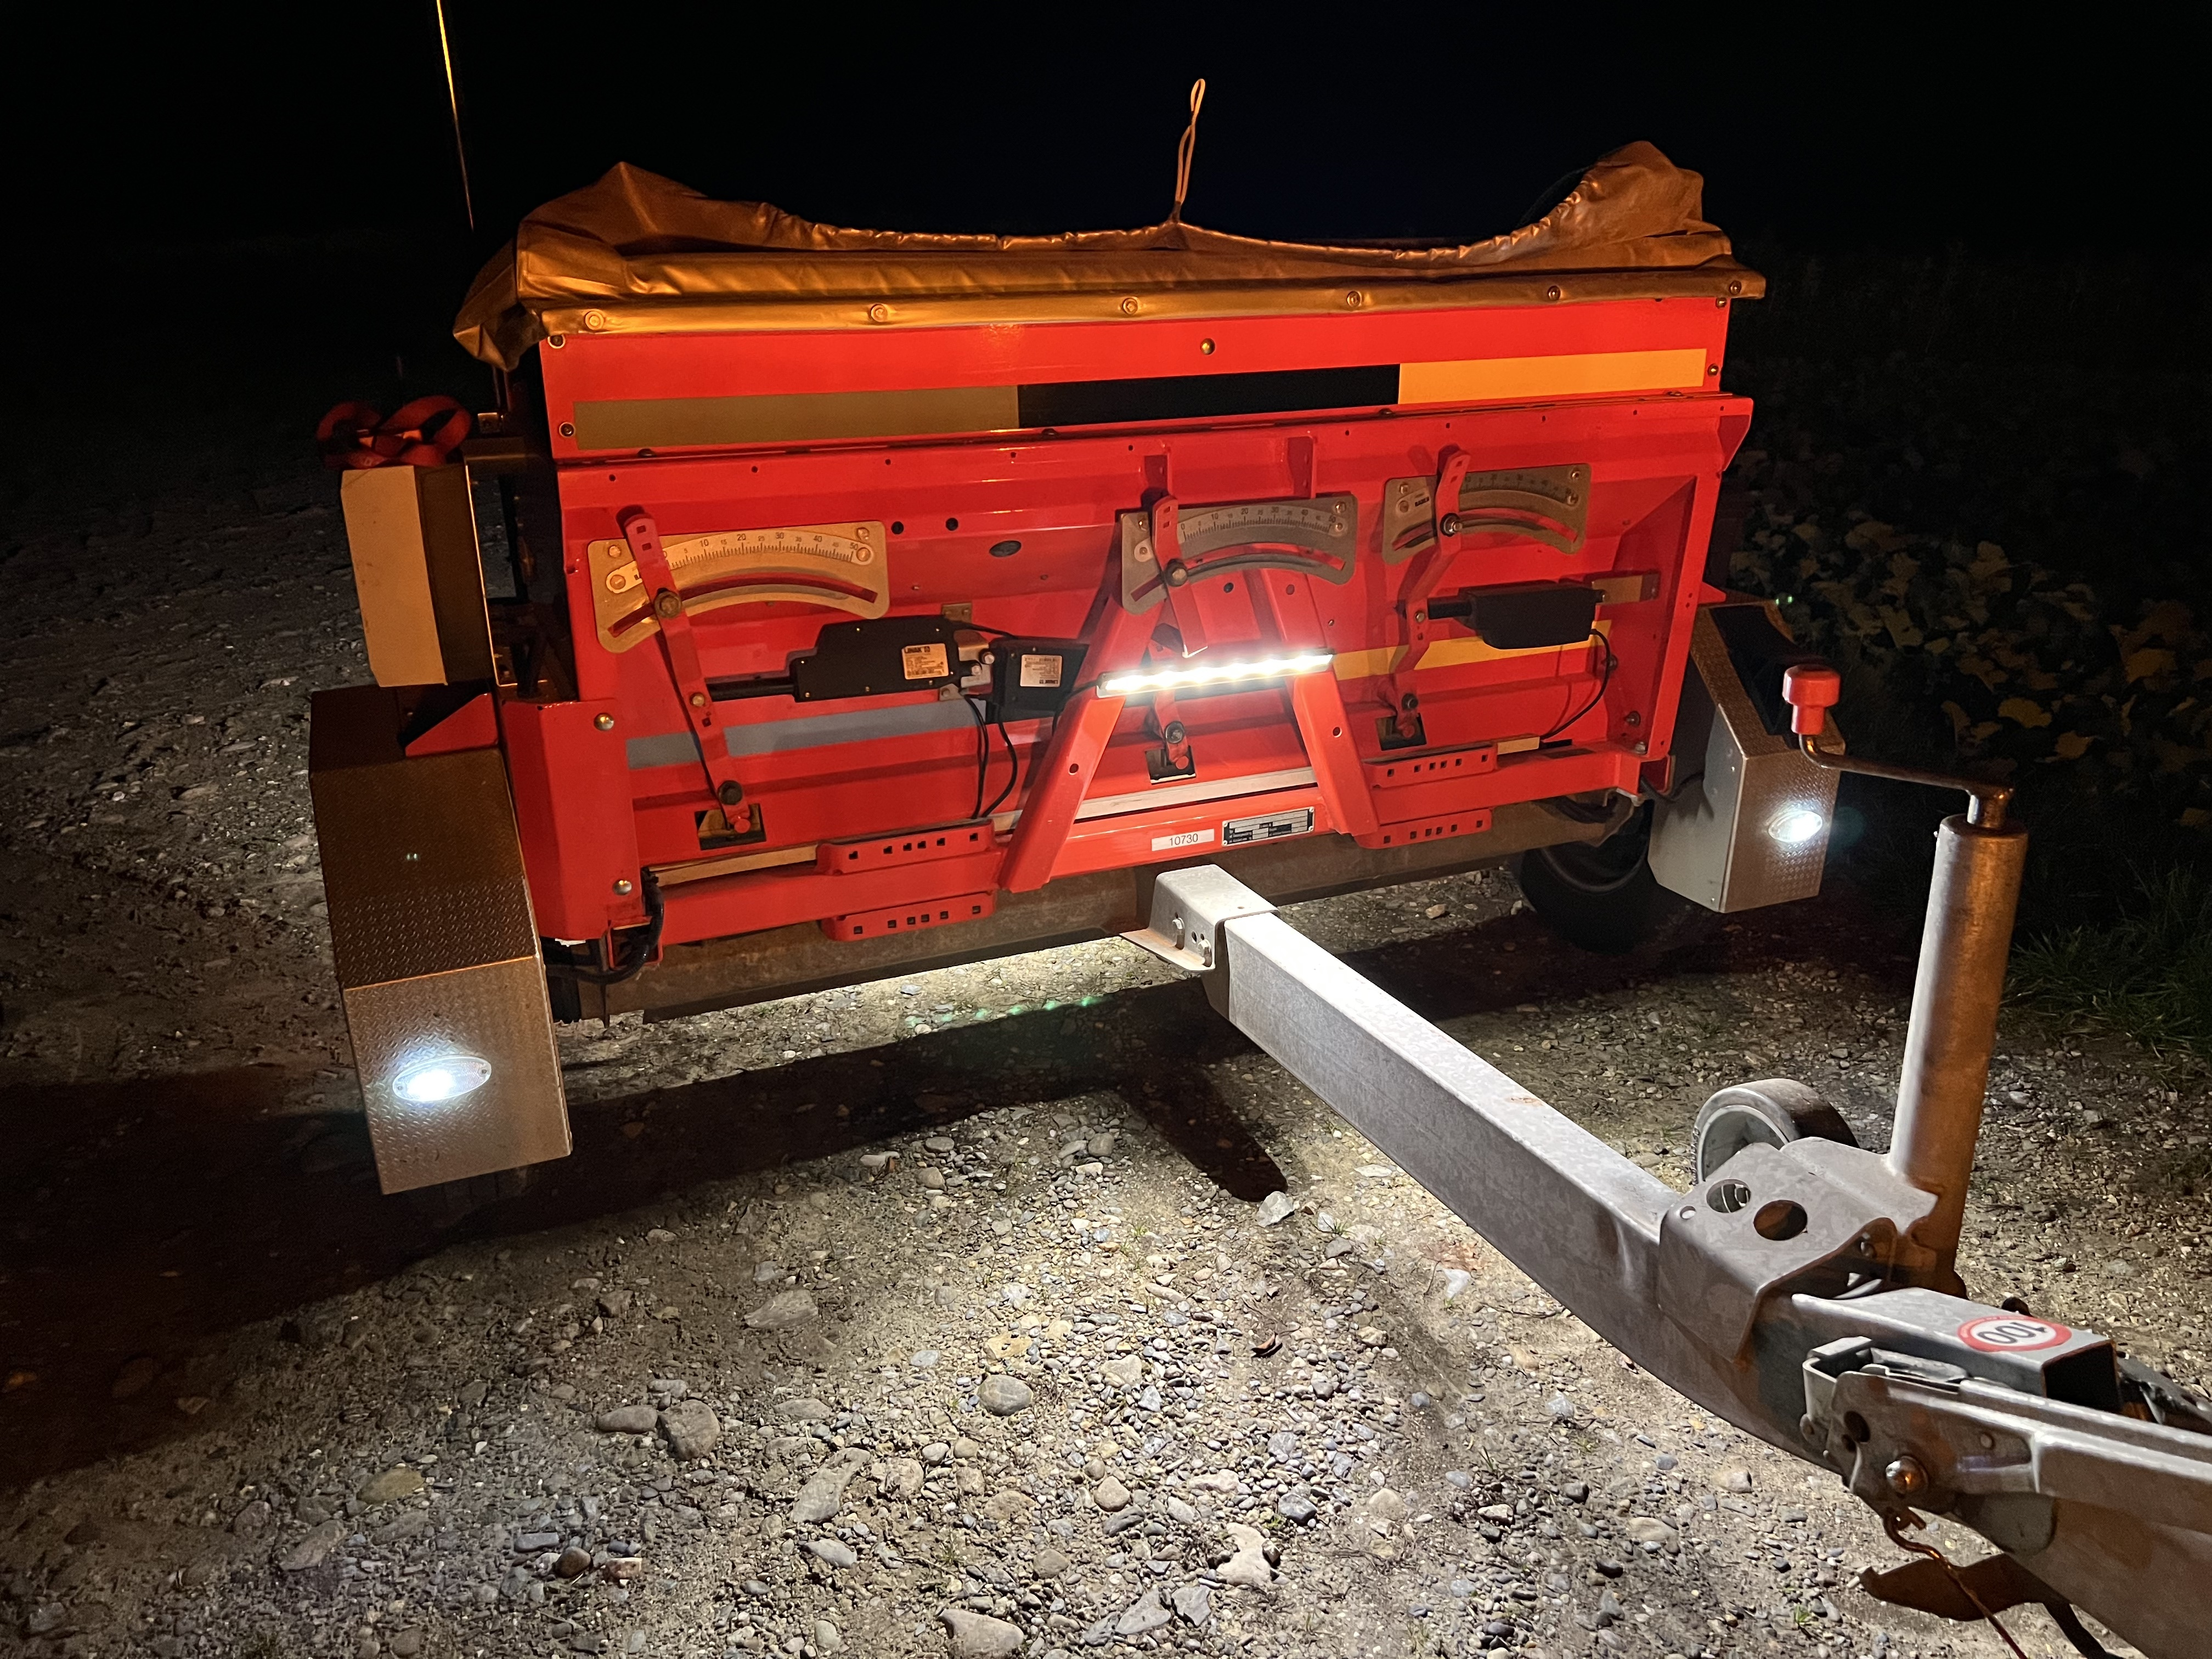
\includegraphics[width=12cm]{assets/figures/remorque.jpeg}
    \caption{Remorque - Vue intérieur}
\end{figure}
\subsection{Caractéristique}
\begin{table}[H]
    \begin{center}
        \caption{Liste de mesure de la remorque}
        \begin{tabular}{|l|l|l|}
            Dimensions                                   & Valeurs                   & Commentaire \\ \hline
            Largeur total des ouvertures                 & 1.50\textbf{[m]}          & [1]         \\
            Largeur d'un semoir                          & 500[mm]                   & -           \\
            Timon - l x H                                & 70 [mm] x 135[mm]         & -           \\
            Timon - hauteur sol                          & 270[mm]                   & -           \\
            Timon - longueur                             & 2.5\textbf{[m]}           & -           \\
            Timon - Distance sans obstacle depuis semoir & 0.8[\textbf{m}]           & -           \\
            Dimensions télécommande L x l x H            & 133[mm] x 62[mm] x 25[mm] & [2]         \\
            Enfoncement des boutons                      & $\sim$ 3-4[mm]            & [3]         \\
        \end{tabular}
    \end{center}
\end{table}

\begin{enumerate}
    \item{Le champ d'action du semoir est beaucoup plus petit qu'une voie de circulation. En Suisse, une voie d'une route cantonale mesure entre 3 et 3.5[m].}
    \item{La télécommande n'est pas parfaitement rectangulaire. Le mécanisme d'activation du l'émetteur de la télécommande occupe la partie gauche de la télécommande,
                si une pression y est exercée, celle-ci ce découple de la commande des semoirs. Il y a également une attache sur la droite de la télécommande.}
    \item{Il y a un "déclique" à atteindre pour actionner les boutons, d'après la mesure qui a été effectuée, il faut une pression de 820 \si{\gram}, ce qui correspond à environ 8 \si{\newton}}.
\end{enumerate}

\begin{figure}[H]
    \centering
    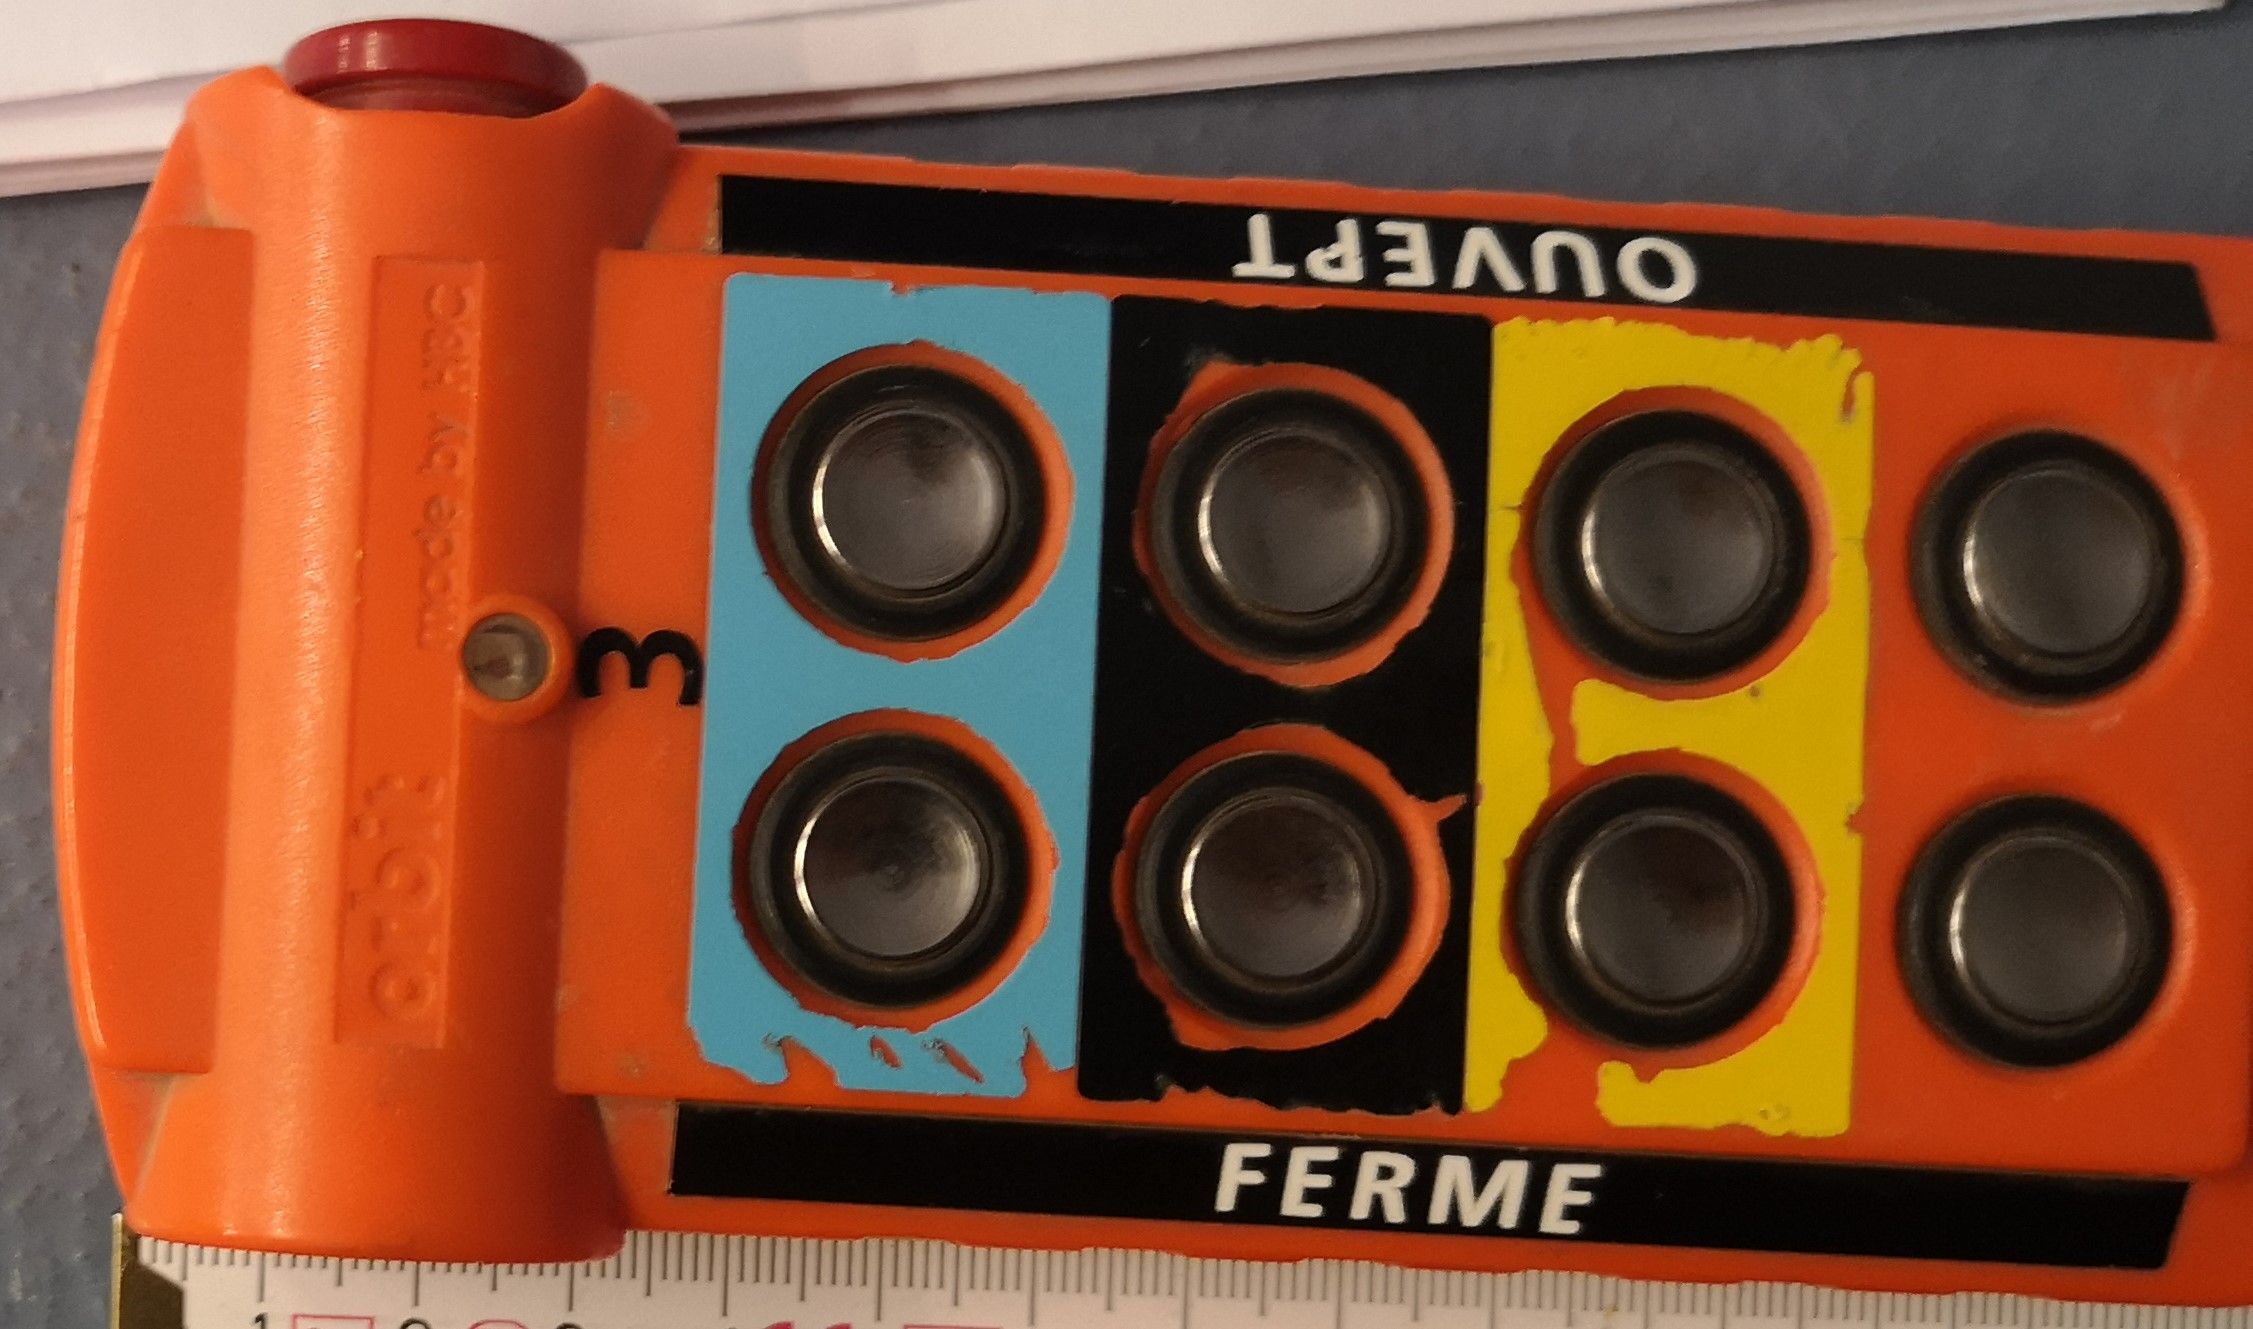
\includegraphics[width=7cm]{assets/figures/telecommande2.jpg}
    \caption{Télécommande - Contrôles des ouvertures}
\end{figure}

\subsection{Alimentation}
Plusieurs sources sont disponibles sur les véhicules tractant la remorque.
\begin{itemize}
    \item{Véhicule 1: 2x prises 13 broches.}
    \item{Véhicule 2: 1x prise 13 broches, 1x prise 7 broches.}
\end{itemize}
A noter que l'installation de base sur la remorque utilise une prise 13 broches.

Il est possible d'avoir du 12 [V] constant sur une prise 13 broches.

\subsection{Fixation}
\subsubsection{Timon de la remorque}
Une partie du timon (environ 80cm) est totalement libre et permettrait d'accrocher du matériel, par exemple un éclairage et/ou une caméra.
Il faudrait malgré tout une fixation adaptée aux dimensions mentionnées dans le tableau de mesure.
\subsubsection{Supports de la remorque}
Il y a deux supports sur la façade intérieure de la remorque, un de chaque côté du timon.
\begin{figure}[H]
    \centering
    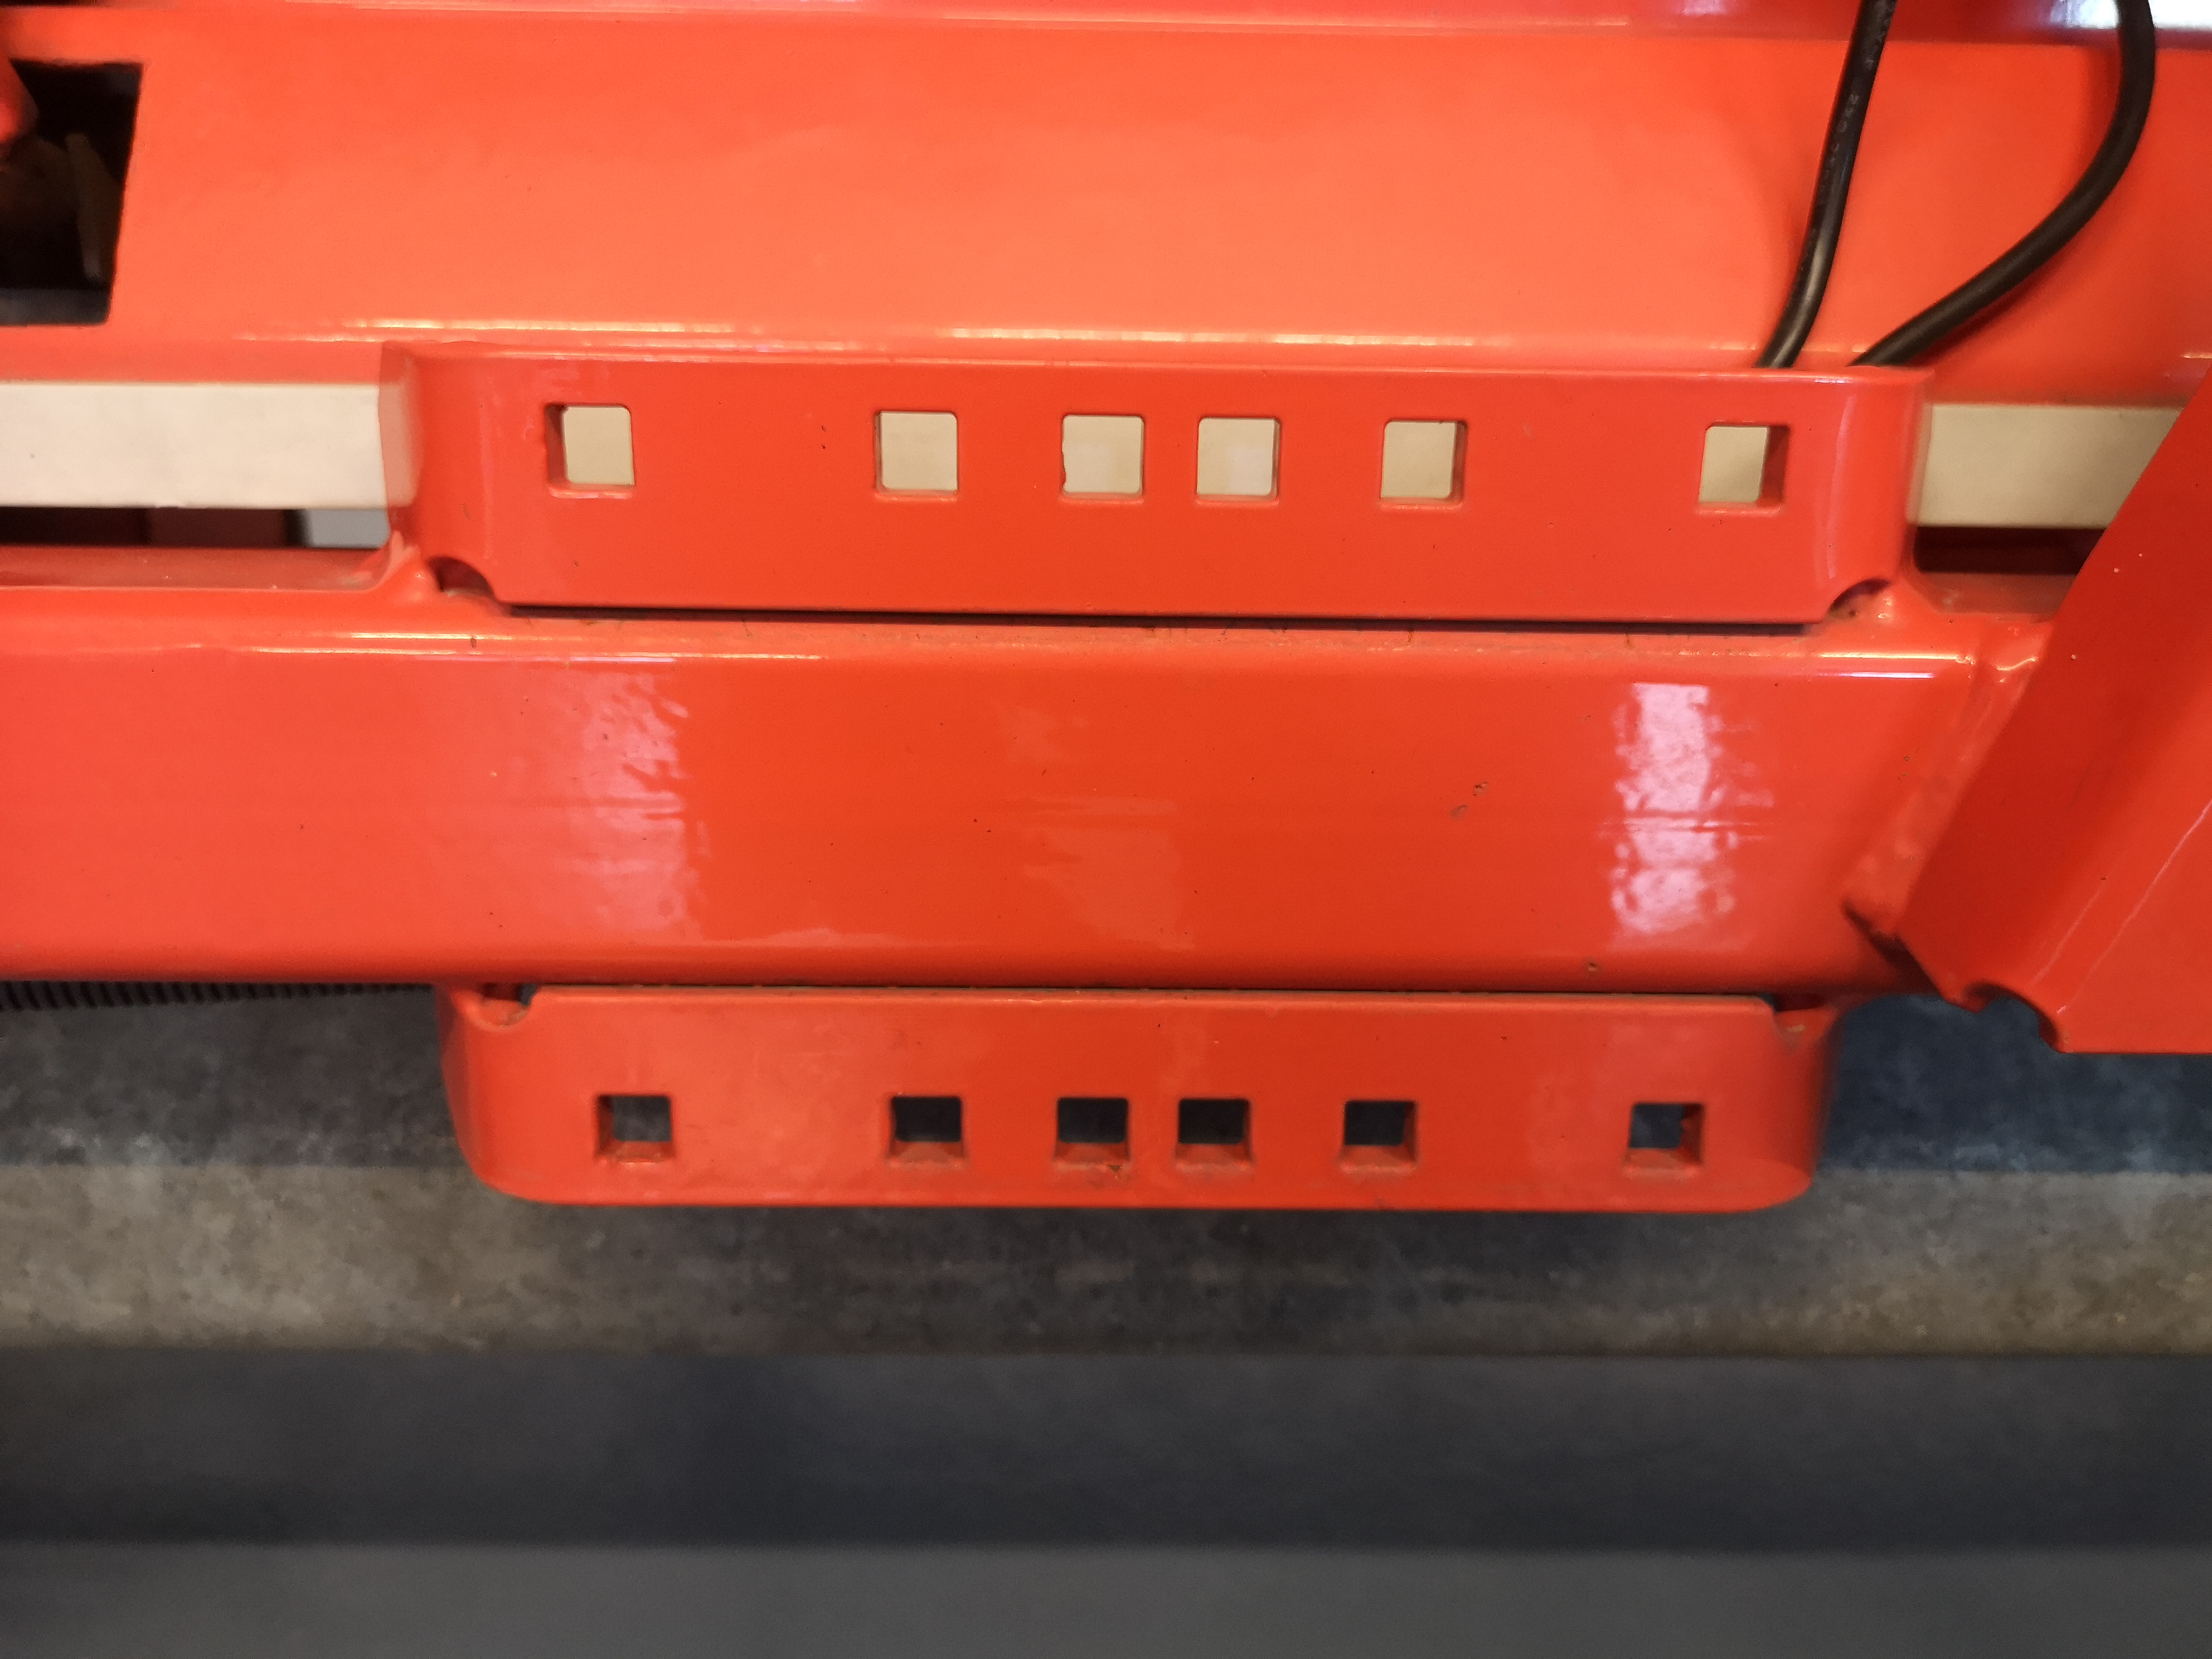
\includegraphics[width=11cm]{assets/figures/support.jpg}
    \caption{Remorque - Support}
\end{figure}

Son emplacement et sa taille pourrait permettre d'y fixer un boitier ou autres éléments relativement facilement.

\chapter{Recherches}
\section{Propriétés réflectives des éléments à capturer}
Durant ses activités, le système observera principalement les éléments suivants:
\begin{enumerate}
    \item Les hydrocarbures
    \item Le béton
    \item Le goudron
\end{enumerate}
En m'informant sur les méthodes de détection déjà existantes des hydrocarbures, j'ai constaté que l'intégralité d'entre eux fonctionnent
par ultraviolet (mesure de fluorescence) et par infrarouge. Je vais donc m'informer sur la réaction des éléments susmentionnés suivant l'exposition à différentes longueurs d'ondes.

\textbf{Note: Le terme "infrarouge" sera noté "IR" dans la suite du rapport.}
\subsection{Hydrocarbures}
Les principaux hydrocarbures traités par les pompiers durant leurs interventions sont les suivants:
\begin{enumerate}
    \item L'huile de moteur.
    \item L'huile hydraulique (tracteur).
    \item L'essence \cite{TotalEnergies}.
    \item Le diesel \cite{TotalEnergies}.
\end{enumerate}
Les éléments principaux qui les composent sont les suivants:
\begin{itemize}
    \item Les alcènes
    \item Les alcanes
    \item Les hydrocarbures aromatiques
\end{itemize}
Divers travaux \cite{Hydrocarbures} traitent des spectres IR des hydrocarbures, mettant en relation la transmittance des éléments en fonction de la longueur d'onde.
Tirés desdits travaux, les graphiques suivants délivres des informations utiles sur la problématique du projet.

\begin{figure}[H]
    \centering
    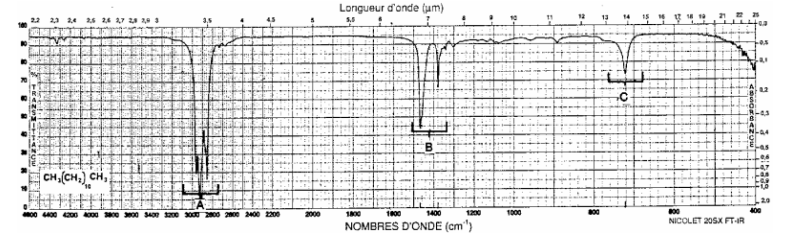
\includegraphics[height=7cm,angle=90]{assets/figures/alcanes1.png}
    \caption{Alcanes - spectre IR du dodécane \cite{Hydrocarbures}}
\end{figure}

\begin{figure}[H]
    \centering
    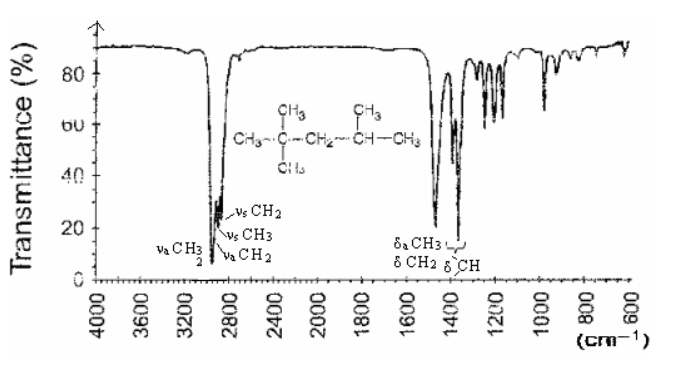
\includegraphics[height=6cm,angle=90]{assets/figures/alcanes2.png}
    \caption{Alcanes - spectre IR du triméthyl-pentane \cite{Hydrocarbures}}
\end{figure}

\begin{figure}[H]
    \centering
    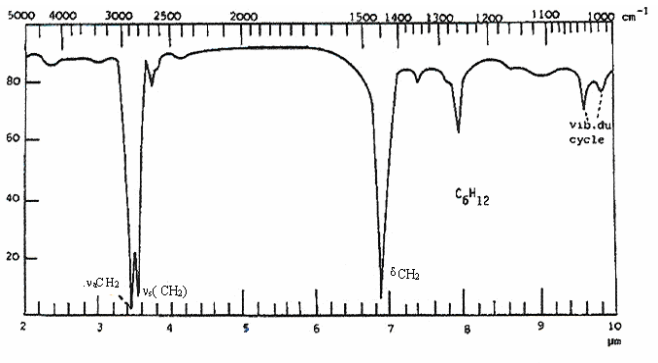
\includegraphics[height=5cm,angle=90]{assets/figures/alcanes3.png}
    \caption{Alcanes - spectre IR du cycloalcanes \cite{Hydrocarbures}}
\end{figure}

\begin{figure}[H]
    \centering
    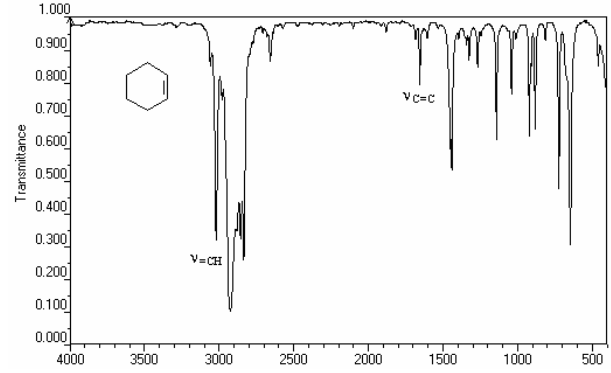
\includegraphics[height=5cm,angle=90]{assets/figures/alcenes1.png}
    \caption{Alcènes - spectre IR du cyclohexène \cite{Hydrocarbures}}
\end{figure}

\begin{figure}[H]
    \centering
    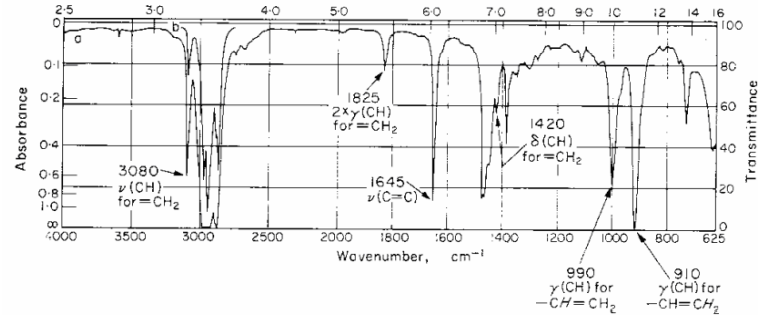
\includegraphics[height=5cm,angle=90]{assets/figures/alcenes2.png}
    \caption{Alcanes - spectre IR du  1-octène à l’état liquide\cite{Hydrocarbures}}
\end{figure}

\begin{figure}[H]
    \centering
    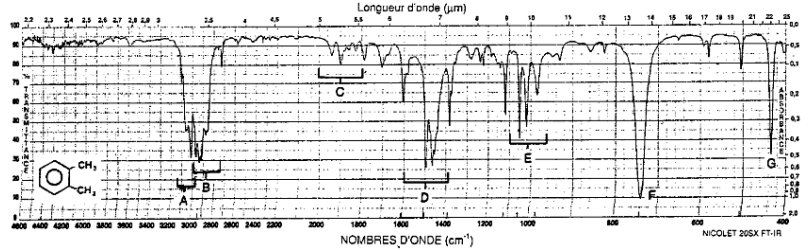
\includegraphics[height=5cm,angle=90]{assets/figures/aromatique.png}
    \caption{Aromatique - spectre IR du o-xylène \cite{Hydrocarbures}}
\end{figure}

\newpage
La transmittance indiquée sur l'axe de l'ordonnée représente l'inverse de l'absorption, c'est à dire que si la transmittance est faible, la lumière
est "très" absorbée par l'hydrocarbure et inversement, si la transmittance est élevée, la lumière est "peu" absorbée par l'hydrocarbure, la laissant ainsi traverser.
Nous observons un point commun pour les trois types d'hydrocarbures, il s'agit des pics d'absorptions aux alentours de \underline{3000 \si{\per\centi\metre}}, ce qui correspond à \underline{3300 \si{\nano\metre}}.

Pour cette longueur d'onde spécifique, la transmittance globale se trouve entre \underline{5 et 30\%}.

\subsection{Route}
Beaucoup de confusion et d'abus de langage sont faites dans les travaux de recherche et dans les documents disponibles sur internet.
Les distinctions entre les matériaux de construction routière sont souvent mal définies ou mal traduites, ce qui entraîne une mauvaise
fiabilité sur les caractéristiques indiquée.
\begin{figure}[H]
    \centering
    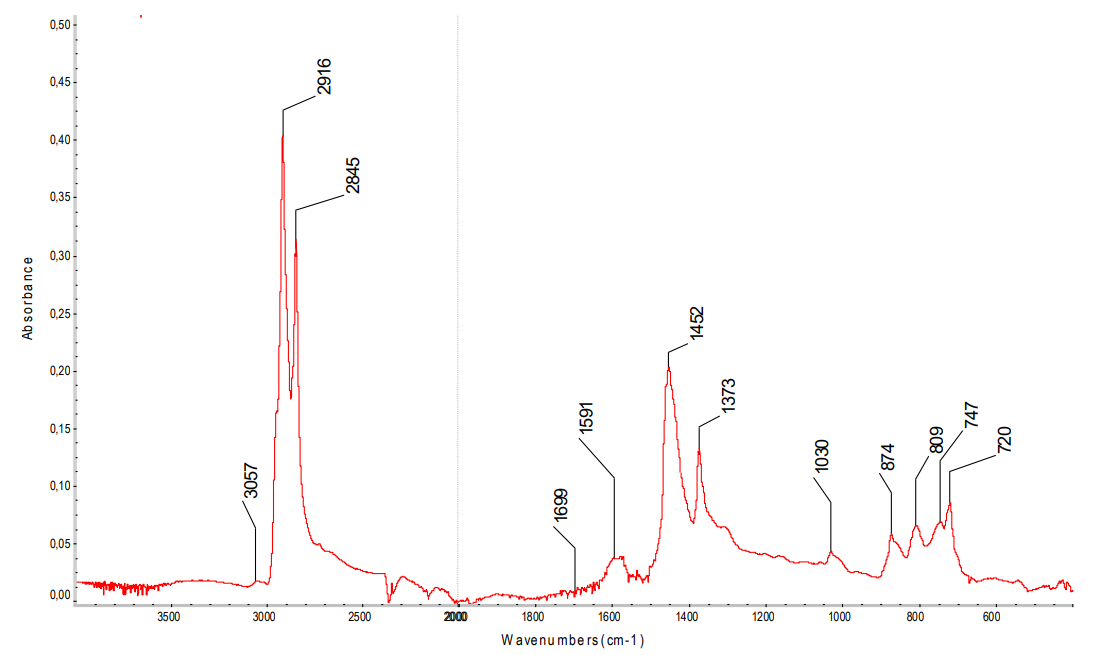
\includegraphics[width=11cm]{assets/figures/bitumeIR.png}
    \caption{Bitume - Spectre IR \cite{Bitume}}
\end{figure}
Ci-dessus un des rares graphe relativement fiable sur le comportement du bitume face aux infrarouges.
\subsection{Analyse}
On observe que les diverses éléments qui seront vus par la caméra ont une variation du taux d'absorptions face aux longueurs d'onde avoisinant les
3300 \si{\nano\metre}, mais à différents ordres de grandeurs. Là ou les hydrocarbures absorbent jusqu'à 95\% des ondes, les routes en absorbent "seulement" jusqu'à 45\%.
En se basant sur ceci, il devrait être possible de faire une différenciation par l'intermédiaire d'un capteur adapté.


Selon les normes \Gls{iso} 20473:2007 \cite{ISO}, cette longueur d'onde se trouve parmi les \Gls{mir}.
\begin{figure}[H]
    \centering
    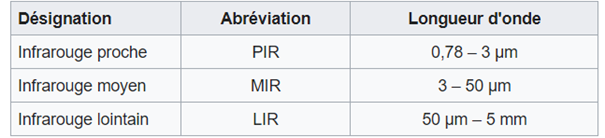
\includegraphics[width=9cm]{assets/figures/gamme_infra.png}
    \caption{Classification des \Gls{ir} selon les normes \Gls{iso} 20473:2007 \cite{ISO}}
\end{figure}

Après des recherches à propos d'un éclairage et surtout d'un capteur adapté à cette gamme de longueur d'onde, je me suis vite aperçu
que les disponibilités et les délais d'arrivées de ce genre de composants ne correspondaient pas avec le rythme d'avancée de mon travail,
j'ai donc exploré d'autres options, toujours dans le milieu de l'infrarouge.

Je suis tombé par hasard sur les produits du "Laboratoire des huiles de moteurs" (faisant parti du HTDS), qui apparemment, utilisent
des rayonnements infrarouges proche du visible (aux alentours de 850nm) pour effectuer des analyses. Très peu de documentation est disponible sur le fonctionnement,
mais la disponibilités d'un capteur et d'éclairage pour cette gamme de longueur d'onde permet d'effectuer des tests très rapidement.
Les résultats de ces tests se trouvent au chapitre \ref{test_vision}.

\textbf{Note suites aux essaies: Les tests semblent concluant et produisent des images exploitables pour effectuer une localisation des
    traces d'hydrocarbures.}

\textbf{\underline{La suite du projet se basera sur un éclairage émettant à 850nm.}}

\chapter{Sélection du matériel}
\section{Alimentation}
Nous avons vu que la remorque utilise une prise 13 broches pour son alimentation. Le véhicule tractant la remorque peut varier, il n'y a donc pas de
garanti qu'il y ait une deuxième prise disponibles pour le système qui sera ajouté. L'idéal serait d'avoir accès au 12[V] et à la masse.
\begin{figure}[H]
    \centering
    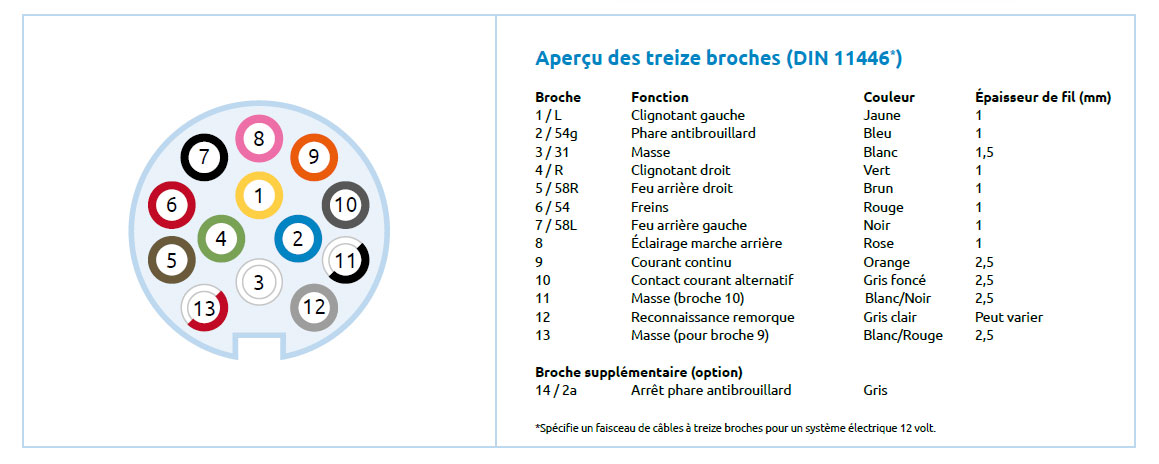
\includegraphics[width=14cm]{assets/figures/broches.jpg}
    \caption{Sortie prises 13 broches - \cite{prise}}
\end{figure}
Ce qui nous intéresse:
\begin{itemize}
    \item Broche 9  : 12 [V]
    \item Broche 13 : Masse
\end{itemize}
Les broches ayant chacune une fonction particulière, il n'existe pas de multiprise permettant de joindre deux connecteurs mâle vers une femelle.
Il faudrait donc fabriquer un boitier d'adaptation ou bricoler une rallonge permettant de dévier les broches utiles, tout en préservant l'alimentation de la remorque et du matériel installé dessus.


Voir figure \ref{alim}.
\begin{figure}[h]
    \centering
    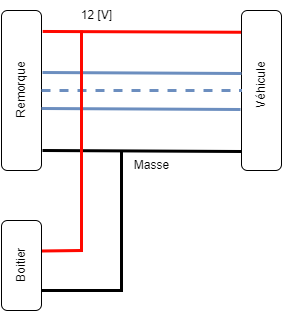
\includegraphics[height=7cm]{assets/figures/alimentation.png}
    \caption{Boitier d'adaptation de l'alimentation \label{alim}}
\end{figure}
\newpage

\section{Communication}
Dans le cadre de ce projet, plusieurs éléments devront communiquer entre eux, notamment l'unité de traitement d'image,
l'actionnement de la télécommande ainsi que le retour vidéo pour le copilote, il est donc important de définir comment ils communiqueront entre eux.
Il est important de se rappeler que leurs emplacements seront les suivants:

\begin{table}[h]
    \begin{center}
        \caption{Liste des éléments et emplacements}
        \begin{tabular}{|c|l|}
            Eléments                        & Emplacement            \\ \hline
            Caméra et boitier de traitement & Support de la remorque \\
            Eclairage                       & Timon                  \\
            Actionnement de la télécommande & Support de la remorque \\
            Affichage pour copilote         & Dans le véhicule
        \end{tabular}
    \end{center}
\end{table}

Dans notre cas de figure, les éléments sont concentrés sur la remorque et dans le véhicule tractant. La communication câblée est possible
entre la caméra, le boitier, l'actionnement de la télécommande et éventuellement l'éclairage si celui-ci à besoin d'être contrôlé spécifiquement.
En ce qui concerne le retour vidéo, il se trouvera principalement dans l'habitacle du véhicule, mais pourrait également être emporté autour du véhicule,
dans ce cas, la connexion filaire n'est pas envisageable.

Parmi les connexions sans fil:
\begin{itemize}
    \item Via une connexion Bluetooth.
    \item Via un réseau \Gls{wifi} local.
\end{itemize}
La connexion sans fil doit garantir une connectivité stable sur un rayon de 5 mètres autour du véhicule (avec obstacles). De plus, le débit doit être
suffisant pour diffuser un flux vidéo. La solution du réseau local \Gls{wifi} semble être la meilleure.

\textbf{La possibilité de communiquer via un réseau local \Gls{wifi} devient donc un prérequis pour le retour vidéo.}
\newpage
\section{Capture et traitement d'image}
\subsection{Eclairage}
La sélection de l'éclairage va dépendre des points suivants:
\begin{itemize}
    \item La longueur d'onde nécessaire.
    \item L'emplacement de l'éclairage
    \item La taille du champ à éclairer.
\end{itemize}
Le premier point s'est défini durant la phase de recherche, l'idéal serait d'avoir une source émettant une onde de 850 \si{\nano\metre}.

Les deux points suivants sont liés, l'éclairage sera monté sur le timon et le but est d'éclairer le sol sur une largeur d'environ 150 \si{\centi\metre} (correspondant aux champ d'actions du semoir),
c'est à dire sur une bande. Avec des leds montées en ligne, il n'est pas nécessaire qu'elles aient un grand angle de diffusion.

Des leds trouvées sur le site de Mouser semblent correspondre à ces conditions \cite{ledIR}.

Leur préparation se résumerait à une mise en bande sur une structure solide (2x 75\si{\centi\metre}) et les alimenter.


\subsection{Caméra}
La caméra à choisir doit remplir les critères suivants:
\begin{itemize}
    \item Pas de filtre IR (ou facilement retirable).
    \item Compatible avec une carte de traitement d'image.
    \item Champ de vision suffisant pour observer la largeur de la route.
\end{itemize}

La caméra Module 3 "NoIR - Wide" de Raspberry Pi \cite{camera} répond aux critères. Avec une mise au point à partir de 5cm vers l'infini,
une résolution de 11.9 mégapixels (4608x2592) et d'un champ de vision de \ang{120}, elle offre une image nette et très détaillée avec beaucoup de liberté sur
son placement. Sa sensibilité aux infrarouges monte jusqu'au environ de 1000 \si{\nano\metre}. Elle est disponible très rapidement et pour 30 \gls{chf}.
\begin{figure}[H]
    \centering
    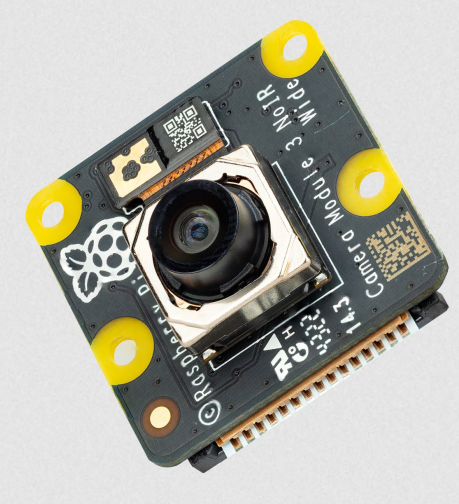
\includegraphics[height=7cm,angle=-90]{assets/figures/camera.png}
    \caption{\href{https://www.digikey.ch/en/products/detail/raspberry-pi/SC0875/17278642}{Camera module 3 NoIR wide}}
\end{figure}
Développement de la largeur nécessaire en pixel en annexe \ref{dev_pxl}.
\newpage
\subsection{Système embarqué de traitement}
L'unité de traitement doit respecter les contraintes suivantes:
\begin{itemize}
    \item Peu encombrant.
    \item Suffisamment puissant pour traiter les images et agir.
    \item Communication WiFi en tant qu'émetteur.
    \item Compatible avec la caméra.
\end{itemize}
En faisant une recherche rapide, on se rend compte qu'il y a beaucoup d'options parmi les marques de nano ordinateur,
et chacune des marques ont une multitude de sous-modèle.
\begin{itemize}
    \item Raspberry Pi.
    \item Intel.
    \item NanoPC.
    \item LattePanda.
    \item NVIDIA.
    \item Et beaucoup d'autres...
\end{itemize}
De manière général, la commande de nano ordinateur est très compliquée actuellement (mars 2023), il faut compter plusieurs semaines voir plusieurs mois
pour espérer recevoir quelque chose. Il est important de noter que j'effectue mon travail de Bachelor à temps plein, en 11 semaines consécutives.
Je ne peux donc pas me permettre d'attendre autant de temps pour recevoir un élément.

En m'informant sur le matériel disponible dans l'école, j'ai appris que le \Gls{reds} prêtait des Raspberry Pi 4.
J'ai donc basé ma sélection sur la disponibilité de l'élément et non pas sur ses capacités.

\textbf{Un Raspberry Pi4 4Go sera utilisé pour la suite du projet.}

Note: Le Raspberry Pi 4 sera abrévié "\Gls{rpi4}" dans la suite du rapport.

\begin{figure}[H]
    \centering
    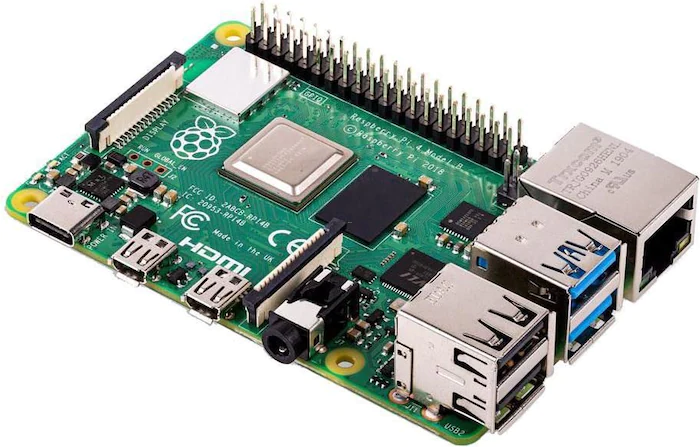
\includegraphics[height=7cm]{assets/figures/rpi4.png}
    \caption{\href{https://www.raspberrypi.com/}{Raspberry Pi4 4Go}}
\end{figure}

\newpage
\section{Système de commande - Actionnement de la télécommande}
Dans le but de conserver le fonctionnement de base du semoir, la commande des vérins se fera par préhension sur la télécommande.
Les idées d'actionneurs sont les suivants:
\begin{itemize}
    \item Vérins électriques.
    \item Servomoteurs.
    \item Moteurs pas à pas.
    \item Aimants de levage.
\end{itemize}

Les vérins électriques ont l'avantage d'être facile à installer, il suffirait d'une plaque de support perforée au dessus de chaque bouton et d'y insérer
les pièces à la profondeur souhaitée, puis de les actionner/rétracter pour appuyer ou non sur un bouton. Cependant, les vérins disponibles sur le marché semblent être surdimensionnés pour la tâche en question, les forces et
consommation pour un fonctionnement normal sont très grand. Les prix sont également très élevé, il est difficile de trouver des pièces de moins de 100 \Gls{chf} l'unité
pour les dimensions désirées. De plus, les délais de livraison durant la période dédiée au développement de se projet sont relativement incertains pour se genre de pièce.

L'idée, avec les servomoteurs, serait de les équiper d'un élément de préhension tangent à l'axe de rotation du moteur permettant de presser sur les boutons.
Le pilotage d'un servomoteur se fait par PWM, nécessitant donc qu'une seule sortie par éléments au niveau de la carte de commande. De plus, il est assez facile de
trouver des servomoteurs avec des caractéristiques en phase avec le projet, c'est à dire d'un point de vu taille, force et consommation, et ce à des prix
raisonnables (avoisinant 10 \Gls{chf}). L'installation sur un support est plus complexe que pour les vérins.

L'utilisation du moteur pas à pas serait similaires au servomoteur, c'est à dire avec un élément qui presse sur les boutons.
Il est assez facile de trouver des moteurs avec des caractéristiques en phase avec le projet à des prix raisonnable (avoisinant 10 \Gls{chf}). La commande d'un moteur pas à pas
se fait usuellement via un pilote servant d'interface entre le moteur et la carte de commande. Il est nécessaire d'avoir une carte pilote par moteur (environ 10 \Gls{chf} par unité).
L'installation sur un support est plus complexe que pour les vérins.

Les aimants de levage, tout comme les vérins ont l'avantage d'être très simple à installer/disposer. Le prix varie suivant la taille, la pression et l'alimentation de l'aimant.
Selon la force nécessaire à l'activation du bouton, le modèle qu'il faudrait utiliser coûte environ 20 \Gls{chf}. L'activation de l'aimant peut se faire via un relai dont le contrôle
pourrait se faire via les pins I/O du \Gls{rpi4}.

Avec ces informations, en comparant prix, facilité d'acquisition, pilotage, caractéristiques obtenables, délai de livraison et facilité d'installation, la solution de l'aimant de levage semble être la plus
appropriée. J'ai trouvé un aimant de levage avec les caractéristiques suivantes:
\begin{itemize}
    \item Tension de fonctionnement: 12 \si{\volt}
    \item Puissance nominale: 7 \si{\watt}
    \item Longueur de déploiement: 10 \si{\milli\metre}
    \item Force en fin de course: 11 \si {\newton}
\end{itemize}

Un test de préhension est effectué au chapitre \ref{aimant}, le test montre que la caractéristique de force de l'aimant n'est pas suffisante.

\section{Retour vidéo}
Le résultat de l'analyse du traitement d'image et la mise en évidence des traces d'hydrocarbures doivent être visible par le conducteur/copilote.
La visualisation du retour se fera naturellement via un écran. Les idées de bases sont les suivantes:
\begin{itemize}
    \item Installation d'un écran portable.
    \item Affichage via une application mobile.
    \item Affichage via une page web locale.
\end{itemize}

Les problèmes de l'écran portable sont multiples, notamment l'alimentation, le câblage vers une source d'alimentation peut-être encombrant
et limiterait les mouvements/déplacements de l'utilisateur. De plus, la connexion vers un réseau \Gls{wifi} local n'est pas garantie.

L'idée de l'application mobile présente certains avantages, comme l'installation unique. L'opérateur n'aurait qu'à mettre l'application
qu'une fois sur son téléphone portable pour accéder au retour vidéo (sous condition d'être connecté au réseau \Gls{wifi} local).
Tout le monde serait alors équiper de son propre écran, petit, pratique et peu encombrant. Le problème majeur est la différence de système d'exploitation
entre les téléphones portables. Le développement d'une application universelle est compliquée, il faudrait avoir une application par système grand public.
De plus, l'installation d'une application non reconnue nécessite des autorisations spéciales sur le téléphone de l'utilisateur.

L'affichage du retour vidéo via une page locale semble être optimal. En plus de regrouper les avantages de l'application mobile, nous nous débarrassons des défauts.
L'accès au lien de la page pourrait se faire via un QR code à scanner sur le boitier de commande.

\textbf{L'affichage se fera via une page web locale.}

\section{Résumé des décisions}
\begin{table}[H]
    \begin{center}
        \caption{Table de résumé des décisions}
        \begin{tabular}{|c|l|}
            Eléments                  & Solutions                         \\ \hline
            Communication             & Filaire + Réseau \Gls{wifi} Local \\
            Eclairage                 & Leds IR 850 \si{\nano\metre}      \\
            Caméra                    & Rpi module 3 NoIR Wide            \\
            Traitement d'image        & Raspberry Pi 4                    \\
            Actionnement télécommande & \textbf{A définir}                \\
            Affichage pour copilote   & Page web local                    \\
        \end{tabular}
    \end{center}
\end{table}
\newpage
\section{Bilan de consommation}
Dans le but d'installer le système sur la remorque, il est important d'avoir une idée de la consommation totale du système afin de dimensionner
un fusible à l'entrée du boitier.

\begin{table}[H]
    \begin{center}
        \caption{Table - Bilan de consommation}
        \begin{tabular}{|c|c|c|c|}
            Eléments                  & Conso. par unité   & Quantité & Conso. totale        \\ \hline
            Camera + \Gls{rpi4}       & 15 \si{\watt}      & 1        & 15    \si{\watt}     \\
            Leds IR                   & 3 \si{\milli\watt} & 100      & 300 \si{\milli\watt} \\
            Actionnement télécommande & -                  & 6*       & -                    \\
            Total                     & -                  & -        & 15.3 \si{\watt}      \\
        \end{tabular}
    \end{center}

    *Normalement, seul 3 actionneurs peuvent être actifs simultanément.
\end{table}

Sachant que l'alimentation depuis la remorque est de 12 \si{\volt}, on en déduit que le courant sera de \(I = P/U = 15.3/12 = 1.275 \si{\ampere} \).
L'utilisation d'un fusible de 1.5 \si{\ampere} semble être une bonne option, cette valeur est disponible au \gls{fablab}. Par la suite, il serait judicieux
d'installer un disjoncteur réarmable afin d'éviter de changer de pièce en cas de problème.

\textbf{À noter que la valeur du courant nécessaire ne tient pas compte des actionneurs de la télécommande. Ce courant devra être recalculé lorsque
    cette aspect sera défini.}

\chapter{Système de vision}
\section{Tests préliminaires \label{test_vision}}
Le but des tests préliminaires est de vérifier que les analyses effectuées dans la phase de recherche sont applicables et nous retournent
des résultats exploitables. Ils permettent également de se rendre compte si le système imaginé lors de la sélection du matériel est en accord avec
ce qui est réalisable.
\subsection{Matériel}
Au moment des tests, les éléments suivants étaient à ma disposition :
\begin{itemize}
    \item 1x Raspberry Pi 4b - 4Go de RAM.
    \item 1x Pi caméra module 3 NoIR Wide.
    \item 20x leds IR 830nm.
    \item 20x leds IR 850nm.
    \item 20x leds IR 880nm.
    \item 1x morceau de route.
    \item 1l. Huile de moteur neuf - 15W-40.
\end{itemize}

\subsection{Eclairage}
L'éclairage utilisé dans le cadre des tests préliminaires consiste en deux rails de leds IR montées en ligne sur deux veroboards.
Le montage a été effectué selon le schéma suivant:
\begin{figure}[H]
    \centering
    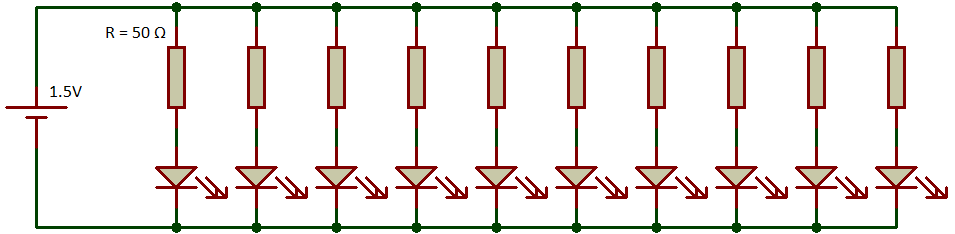
\includegraphics[width=13cm]{assets/figures/schema_leds1.png}
    \caption{Eclairage de test - Schéma électrique de la rangée de led - Schéma modifié de: \url{https://www.sonelec-musique.com/electronique_realisations_alim_led.html}}
\end{figure}
Les veroboards sont pratiques à manipuler, il est possible se les tenir avec des étaux afin de faire varier les positions durant les tests. Une fois monté,
le résultat est le suivant:
\begin{figure}[H]
    \centering
    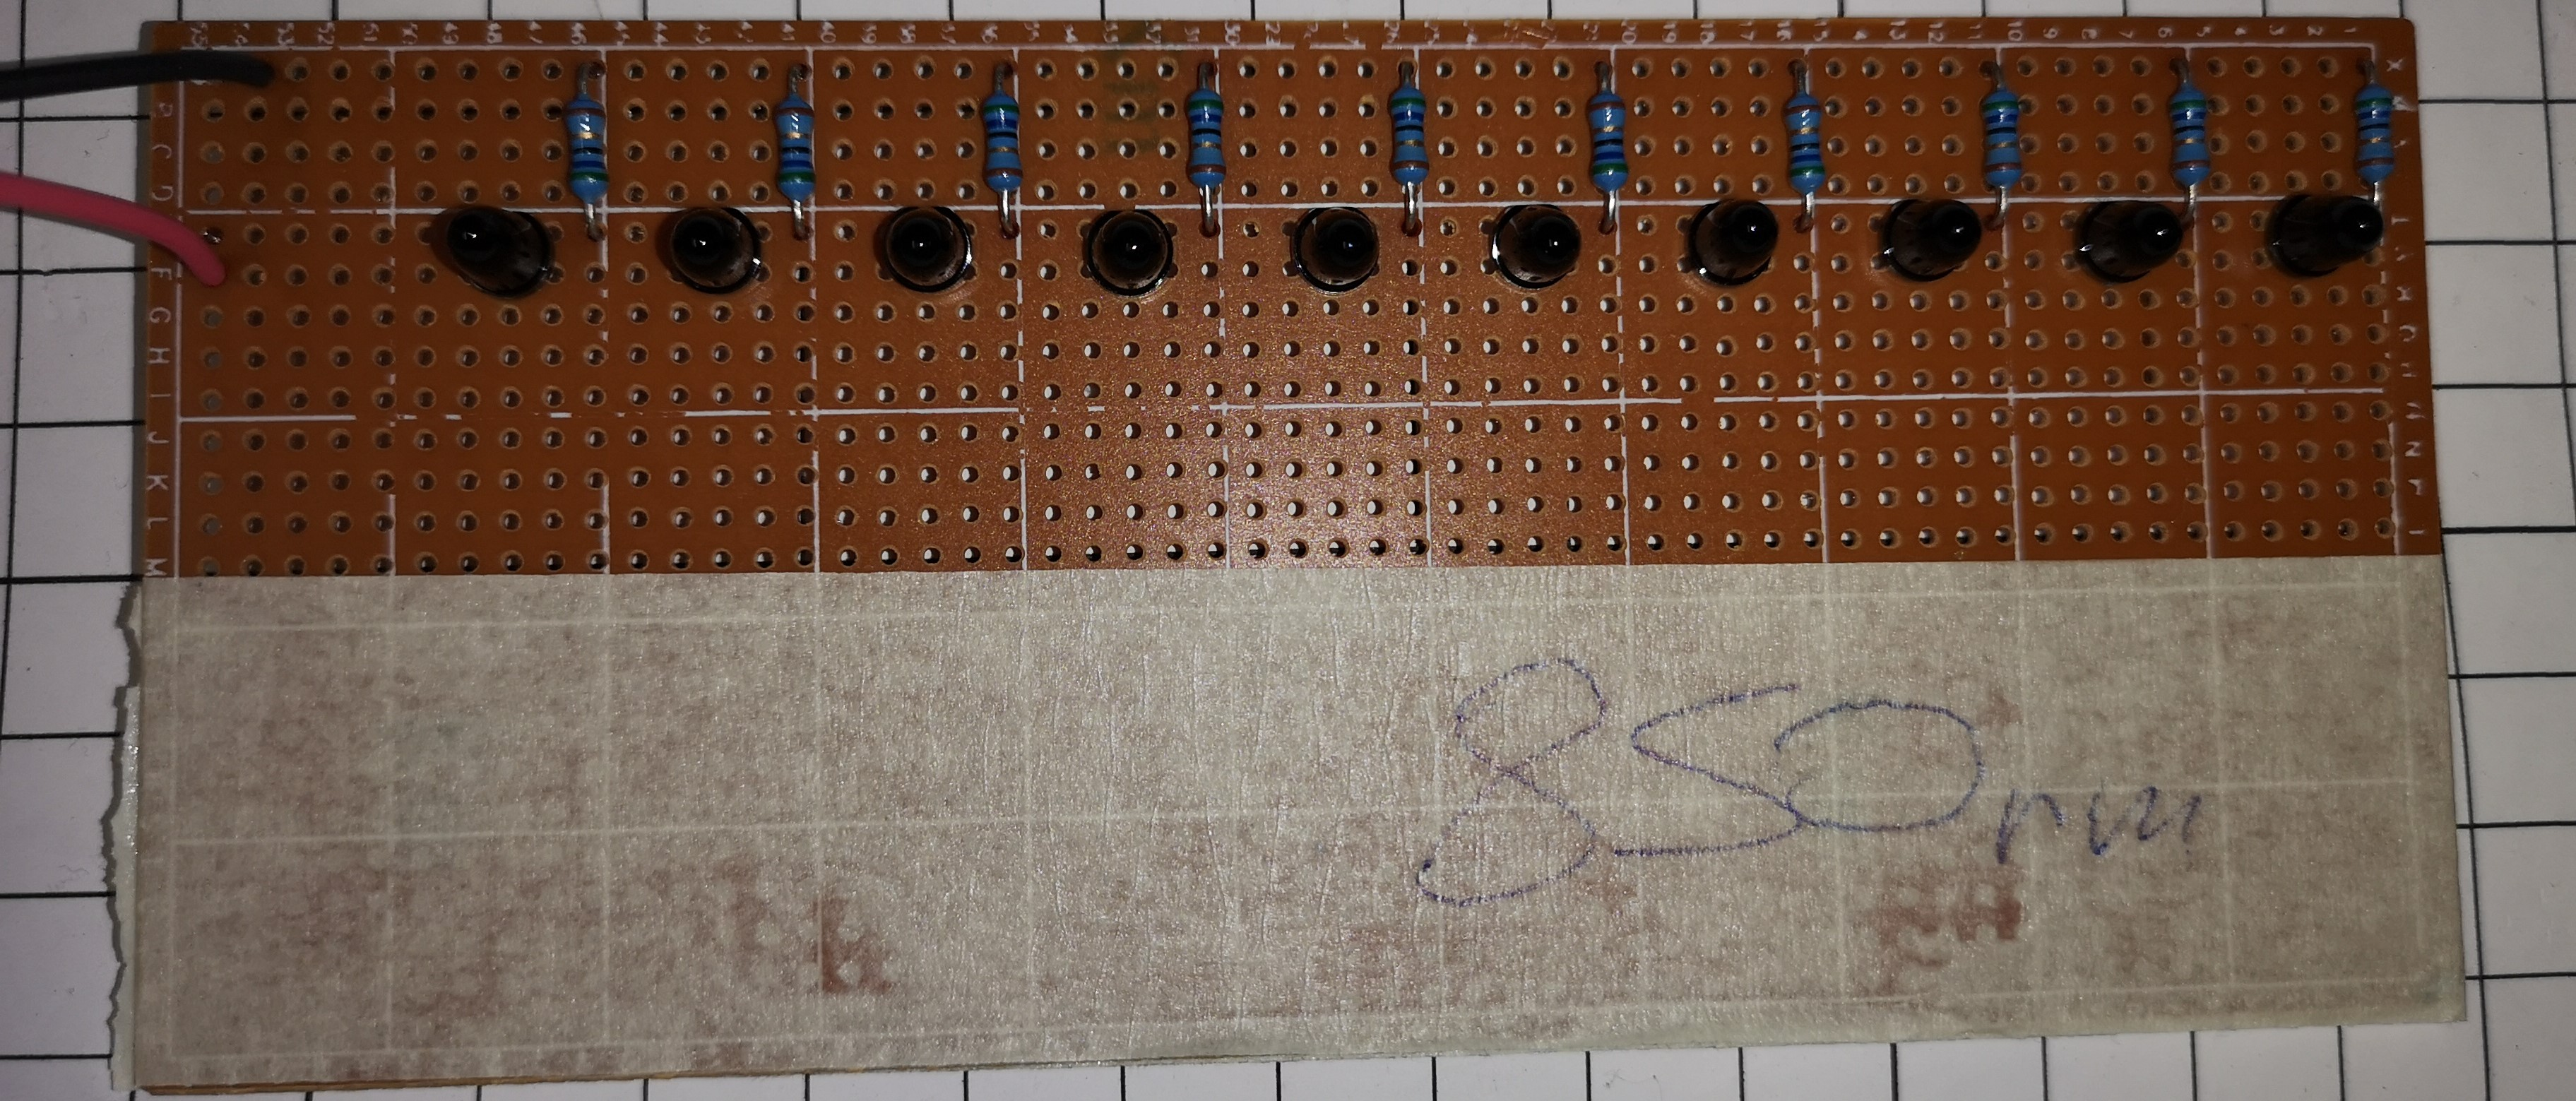
\includegraphics[width=13cm]{assets/figures/rail_led1.jpg}
    \caption{Eclairage de test - Rail de leds 1}
\end{figure}

\begin{figure}[H]
    \centering
    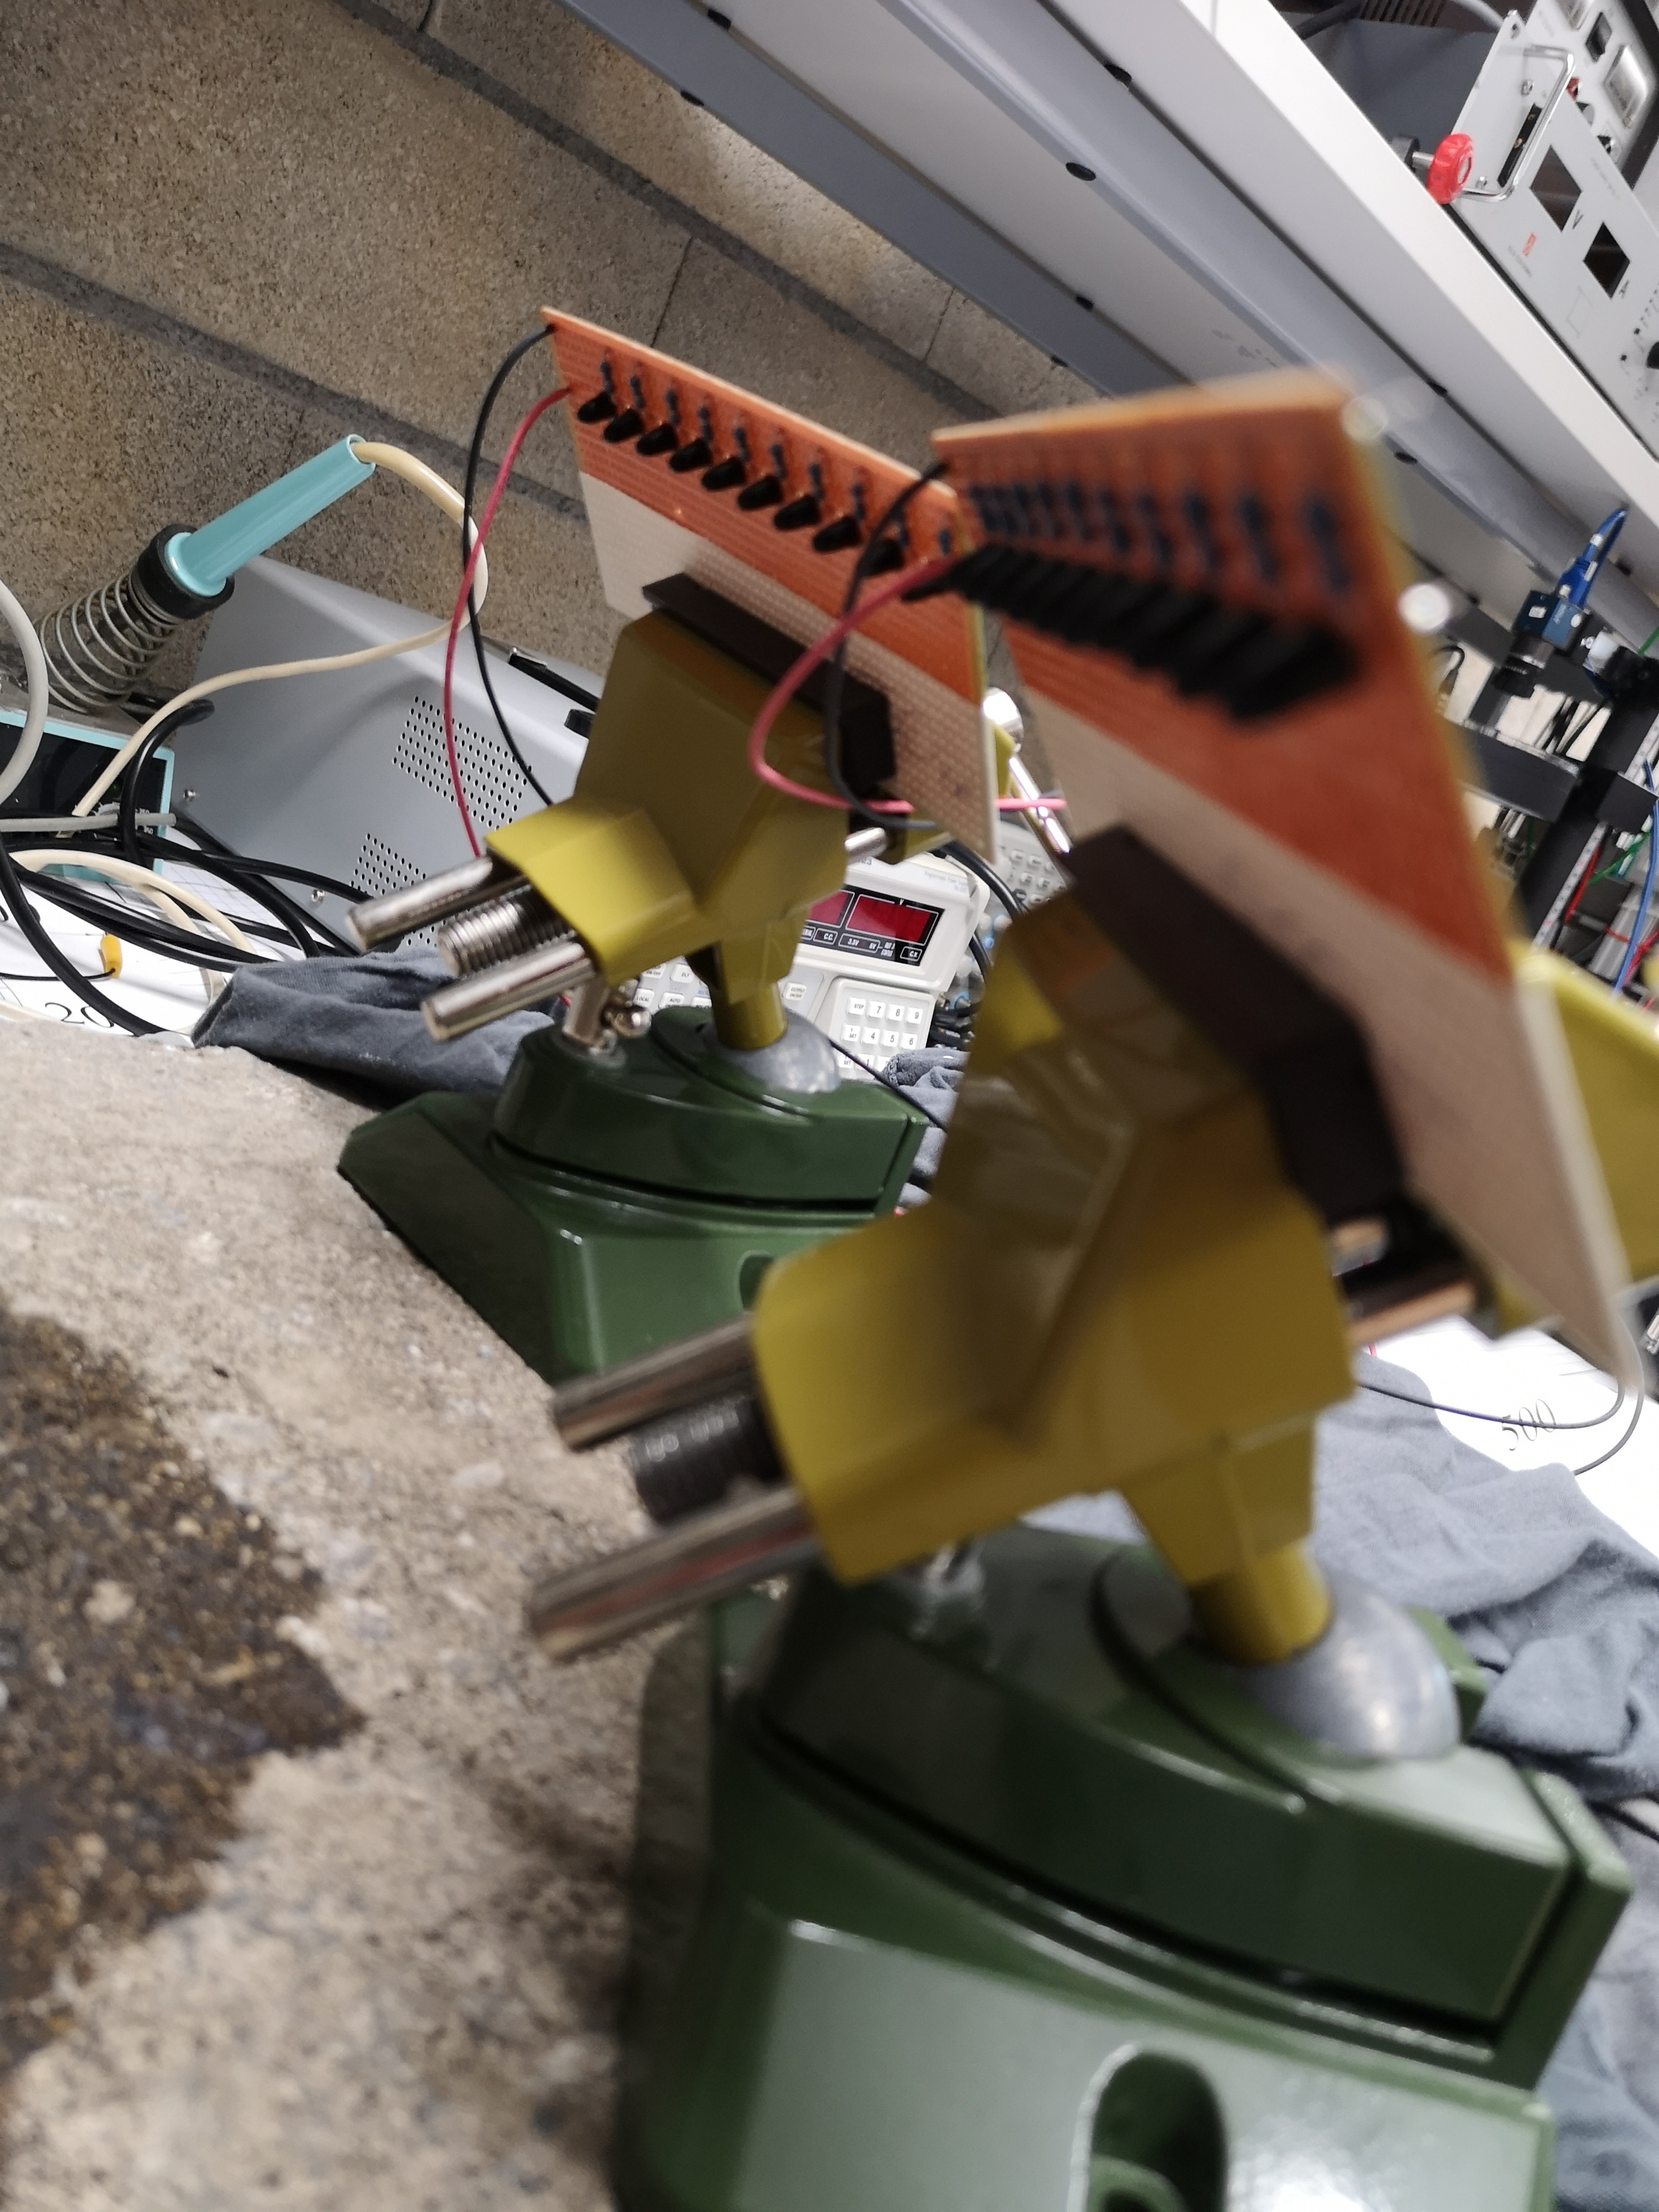
\includegraphics[width=8cm]{assets/figures/rail_led2.jpg}
    \caption{Eclairage de test - Rail de leds 2}
\end{figure}
\subsection{Capture}
La capture d'acquisition des images de tests préliminaires se fait via la caméra sélectionnée durant la phase de décision, un Rpi4 ainsi
qu'un petit script configurant la caméra et enregistrant l'image.
\subsection{Images}
Vu depuis la caméra, nous avons la scène suivante:

\begin{figure}[H]
    \centering
    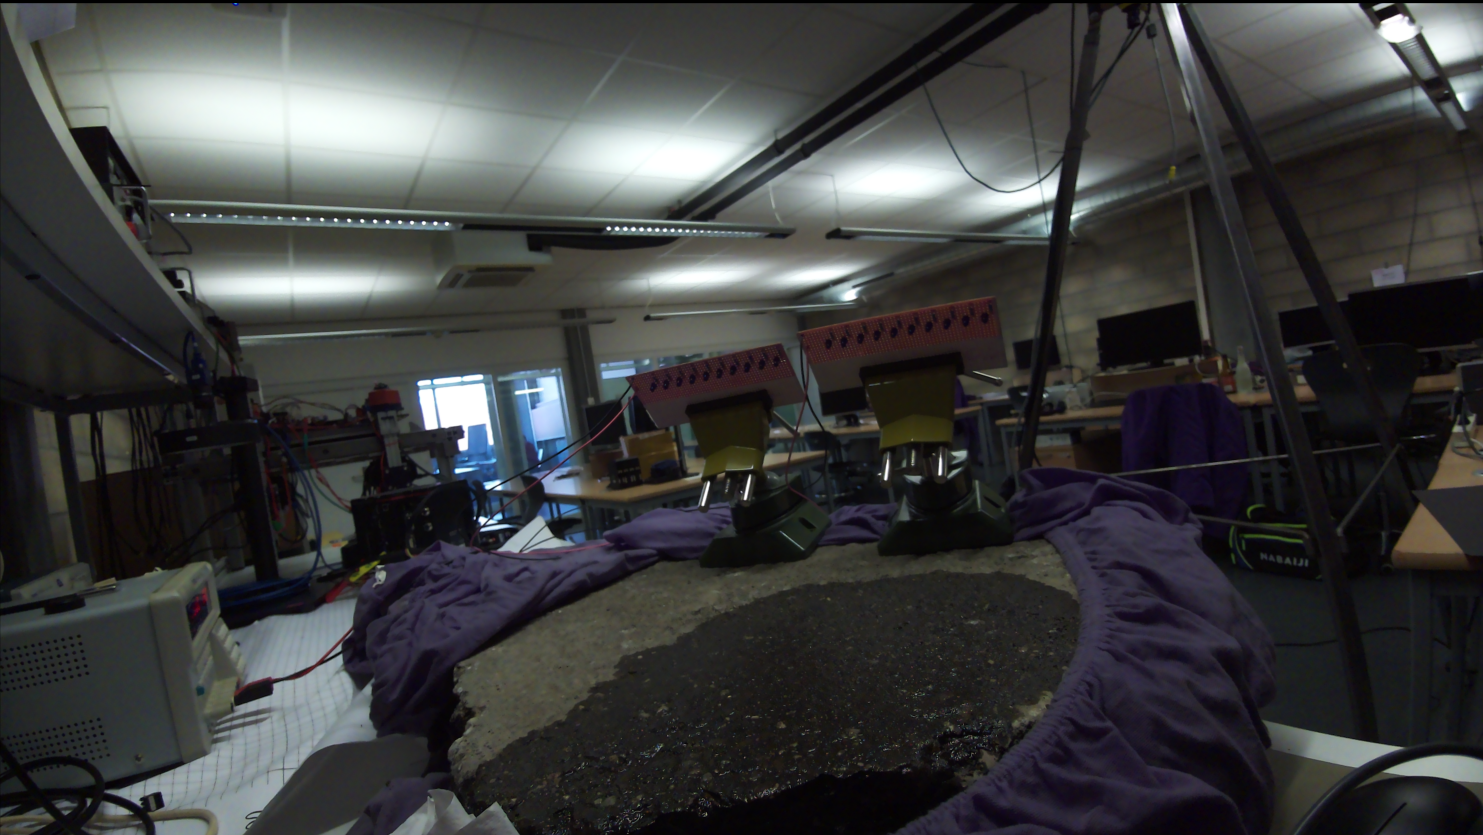
\includegraphics[width=13cm]{assets/figures/camera_vue_couleur1.png}
    \caption{Capture de test - Vue de la scène en couleur}
\end{figure}

Au moment d'effectuer les tests de sensibilités aux IR, tout le matériel n'était pas encore arrivé, notamment le filtre de l'objectif ne
laissant passer que les infrarouges. J'ai donc effectué les captures qui vont suivre dans les conditions suivantes:
\begin{itemize}
    \item Lumières éteintes dans la pièce.
    \item Deux lignes de 10 leds IR éclairant en direction de la tâche d'huile de moteur.
    \item Protection contre les lumières parasites du couloir (carton).
    \item Auto-focus sur le centre de l'image
    \item Temps d'exposition: 5000[ns]. (déterminé expérimentalement avec plusieurs captures)
\end{itemize}
Avec ce setup, j'ai effectué plusieurs captures en faisant varier la position de l'éclairage par rapport à la tâche d'huile et la caméra.
J'ai obtenu différents résultats, plus ou moins utilisables.


Ci-dessous, un exemple d'éclairage orienté "contre" la caméra selon la figure suivante:
\begin{figure}[H]
    \centering
    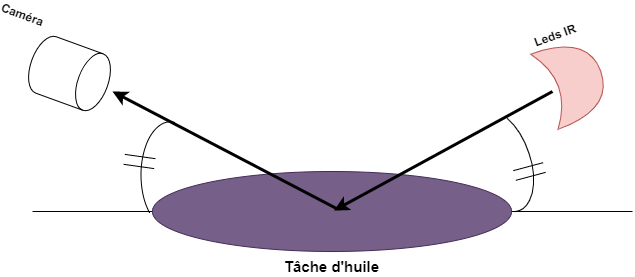
\includegraphics[width=13cm]{assets/figures/eclairage_contre_camera.png}
    \caption{Schéma de capture - Eclairage contre la camera \label{led_perp}}
\end{figure}


\begin{figure}[H]
    \centering
    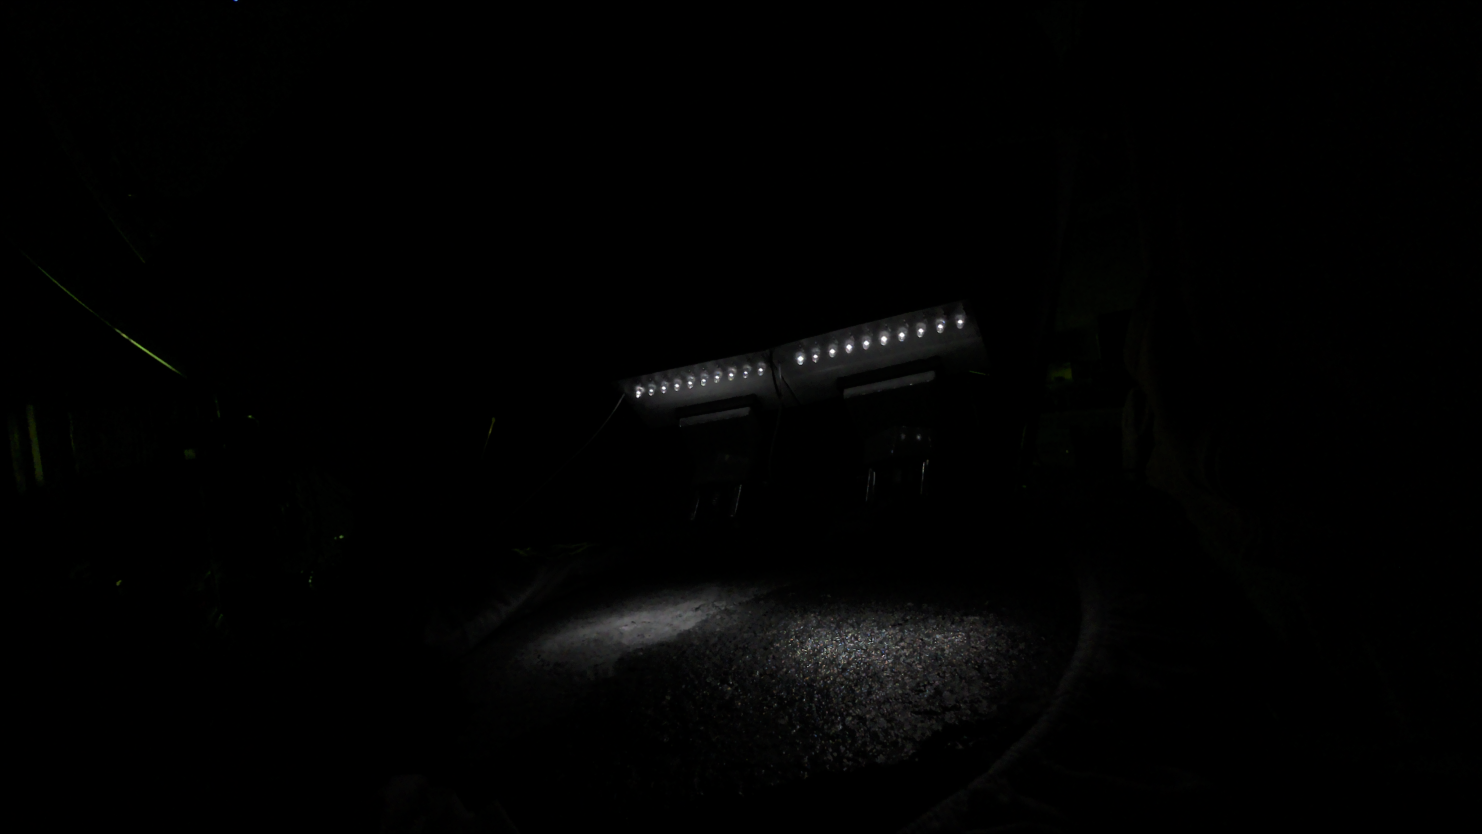
\includegraphics[width=13cm]{assets/figures/eclairage_face1.png}
    \caption{Capture de test - éclairage de face 1}
\end{figure}
\begin{figure}[H]
    \centering
    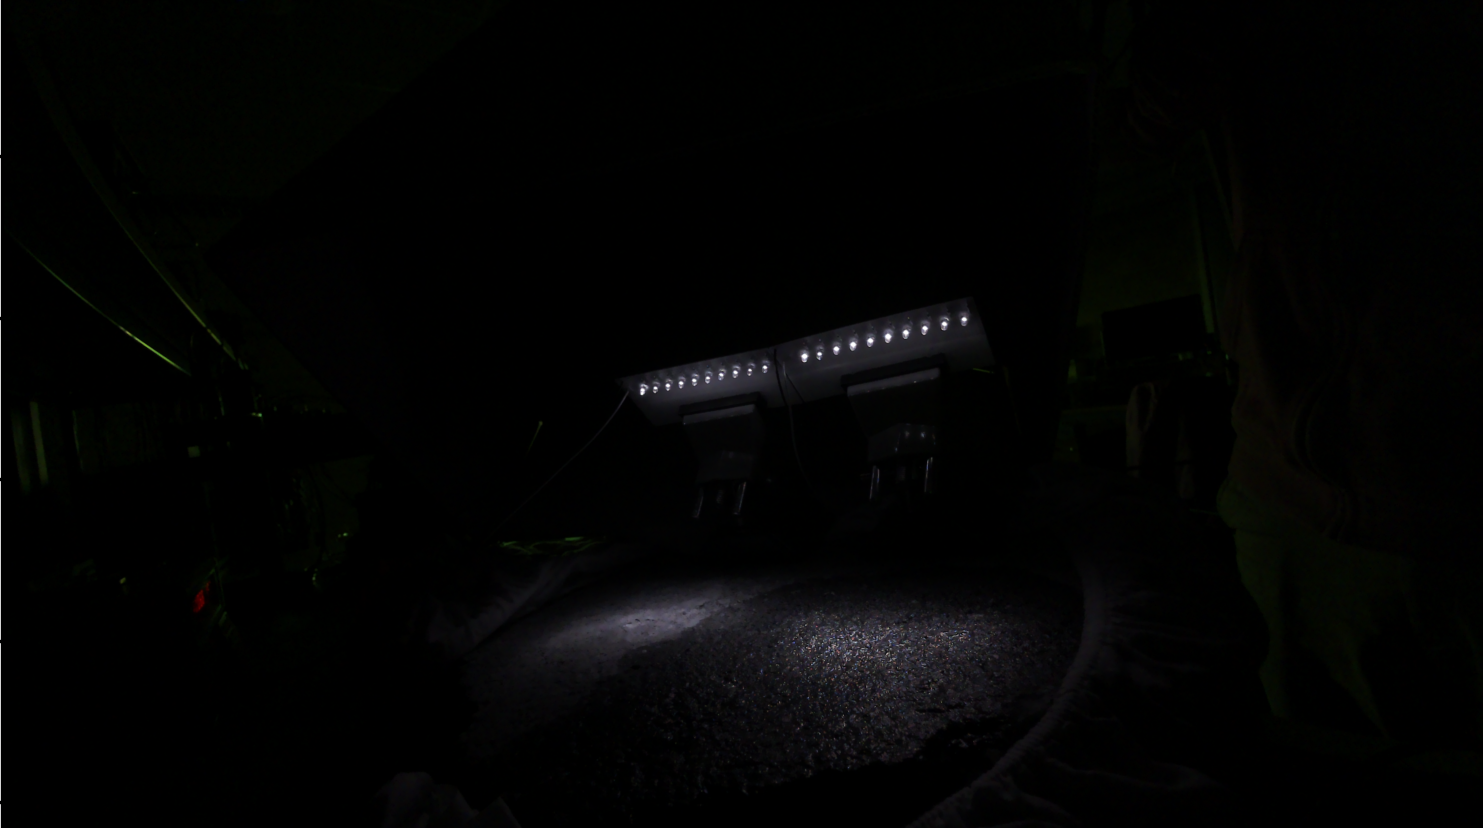
\includegraphics[width=13cm]{assets/figures/eclairage_face2.png}
    \caption{Capture de test - éclairage de face 2}
\end{figure}

On observe que la route et l'huile reflètent les leds IR, à l'oeil nu la différence est notable, mais l'analyse avec un soft peut s'avérer compliquée.\\
Ci-dessous, un exemple d'éclairage orienté perpendiculairement à la route selon la figure suivante:
\begin{figure}[H]
    \centering
    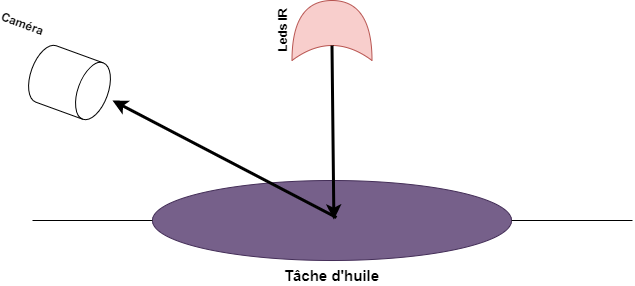
\includegraphics[width=13cm]{assets/figures/eclairage_perpendiculaire.png}
    \caption{Schéma de capture - Eclairage perpendiculaire à la route}
\end{figure}

\begin{figure}[H]
    \centering
    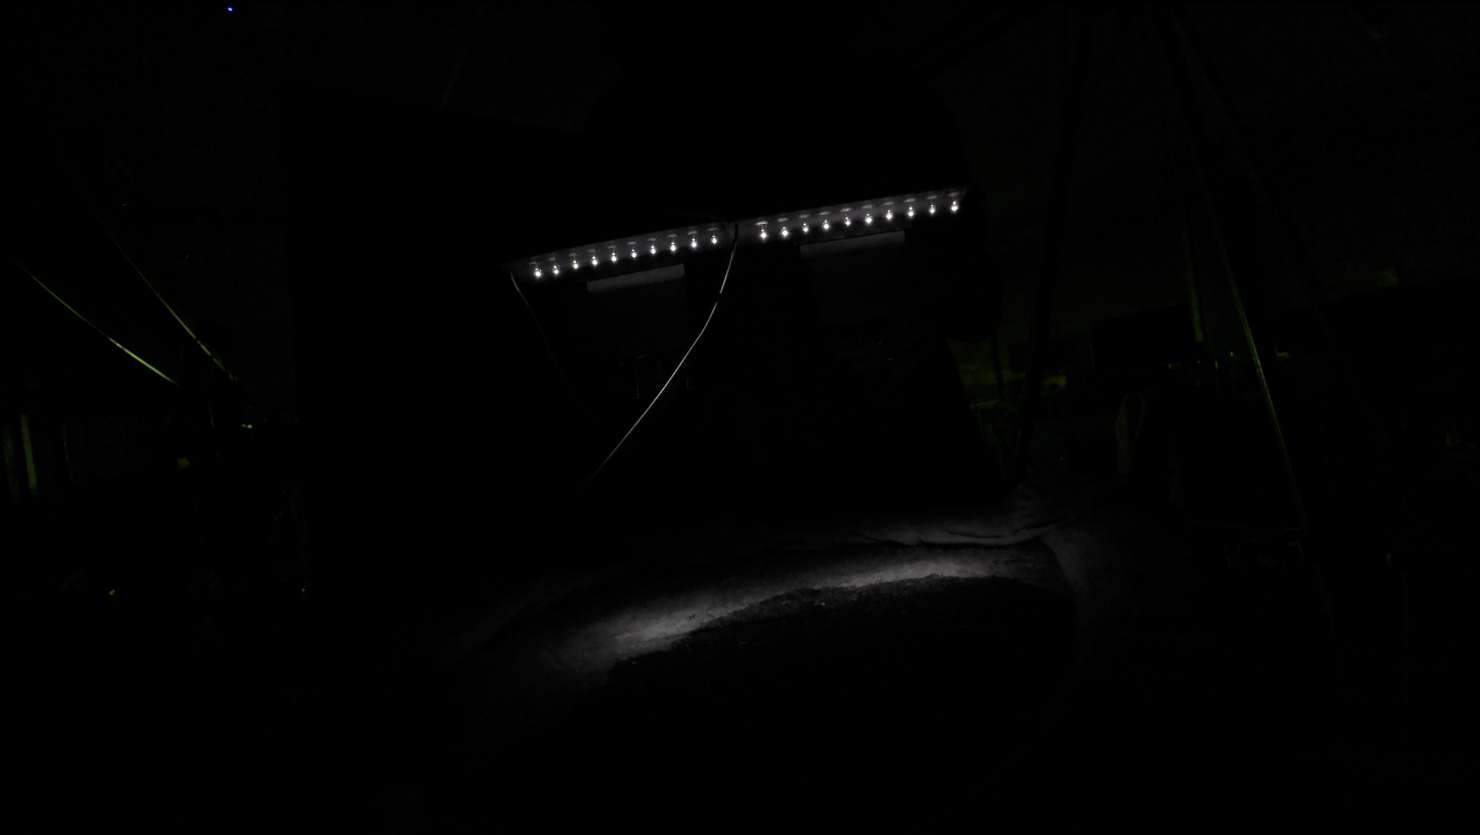
\includegraphics[width=13cm]{assets/figures/eclairage_perpendiculaire1.png}
    \caption{Capture de test - Eclairage perpendiculaire 1}
\end{figure}
\begin{figure}[H]
    \centering
    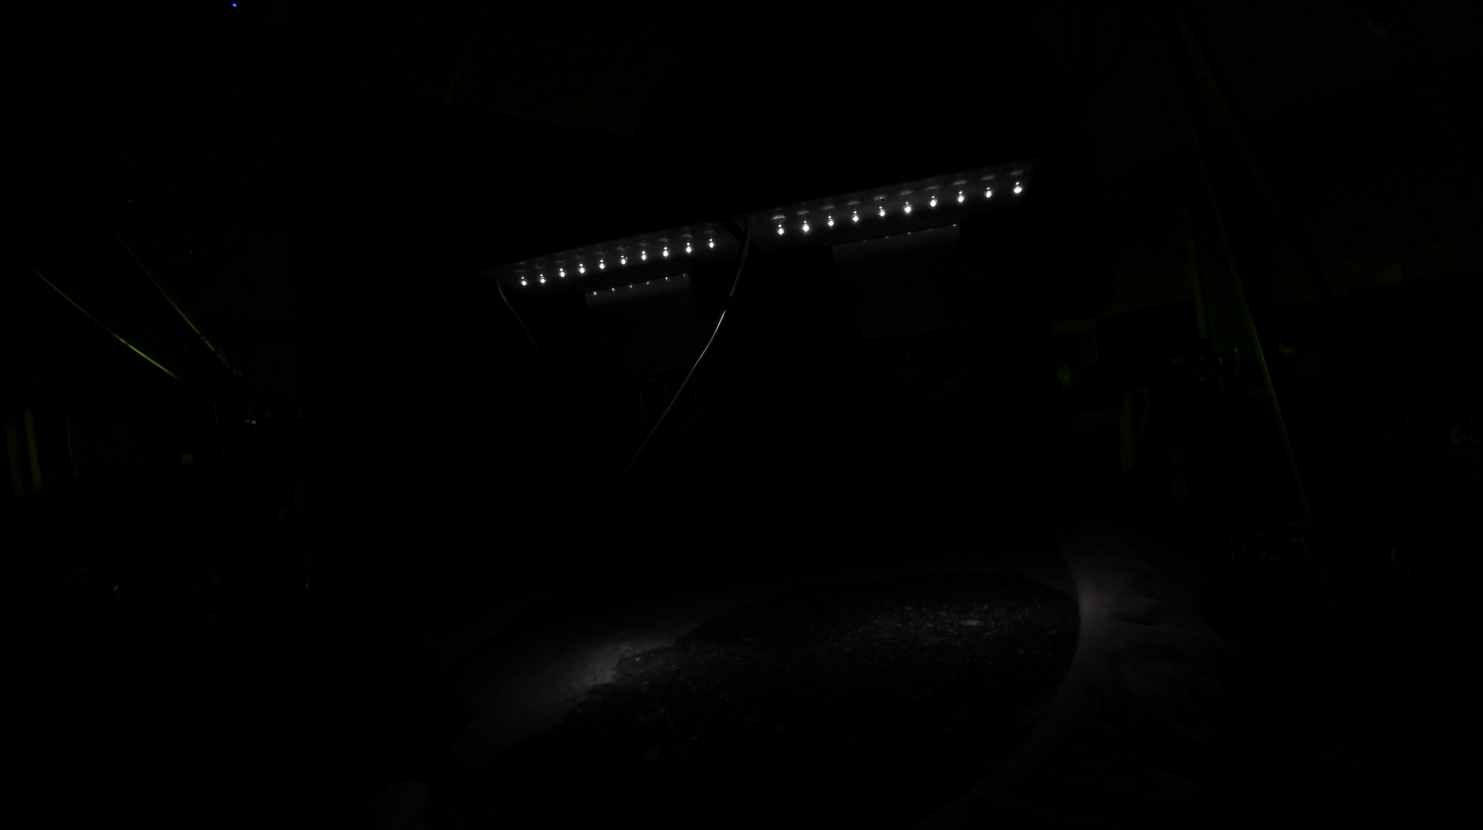
\includegraphics[width=13cm]{assets/figures/eclairage_perpendiculaire2.png}
    \caption{Capture de test - Eclairage perpendiculaire 2}
\end{figure}

\begin{figure}[H]
    \centering
    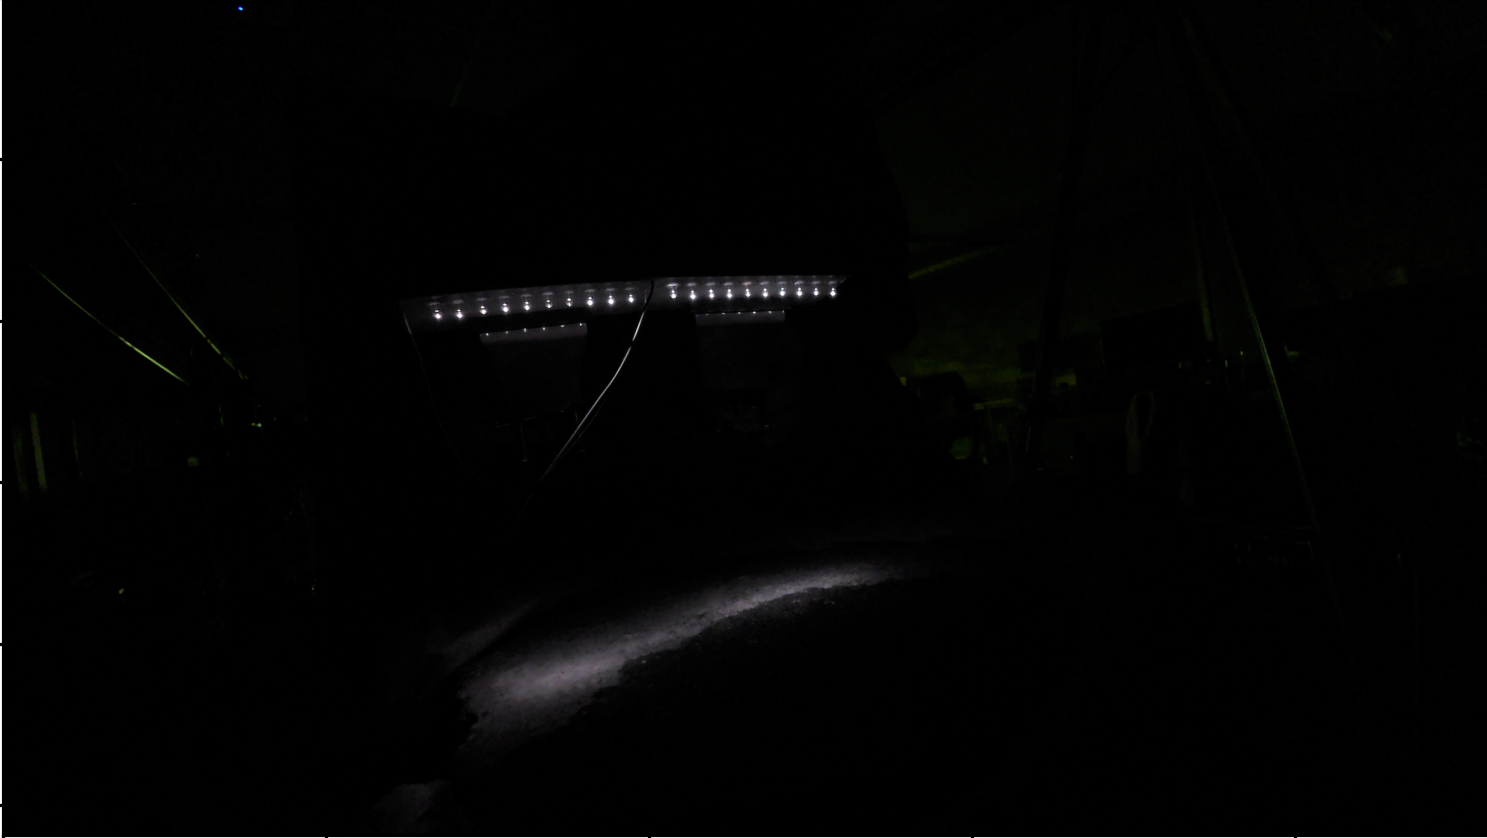
\includegraphics[width=13cm]{assets/figures/eclairage_perpendiculaire3.png}
    \caption{Capture de test - Eclairage perpendiculaire 3}
\end{figure}
On observe que la route diffuse, dans une moindre mesure, l'éclairage des leds IR, là ou l'huile semble absorber les rayonnements. On arrive
assez facilement à différencier le clair de la route et le foncé de l'huile. La mise en place d'un software de détection est envisageable avec
un éclairage basé sur ce schéma. A noter que les tests ont été effectués avec plusieurs gammes de leds (830nm, 850nm et 880nm), la différence
sur le retour image n'est pas très grandes, mais les leds 850nm permettent de mieux différencier la route de l'huile.
\newpage
J'ai également tenté la configuration suivante:
\begin{figure}[H]
    \centering
    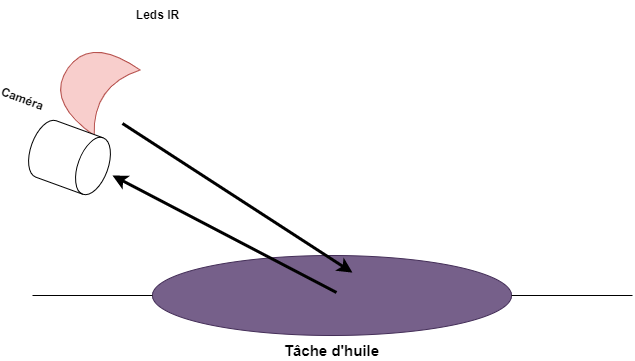
\includegraphics[width=13cm]{assets/figures/eclairage_dos.png}
    \caption{Schéma de capture - Eclairage de dos}
\end{figure}
Mais, étant trop sombre, les images obtenues n'étaient pas utilisables.
\newpage
\subsection{Filtre du visible}
J'ai effectué quelques tests supplémentaires après la réception des filtres ne laissant passer que l'infrarouge. Pour rappel, le filtre
ne laisse passer que les ondes supérieures à 700nm, les rouges lointains seront encore visibles.

\begin{figure}[H]
    \centering
    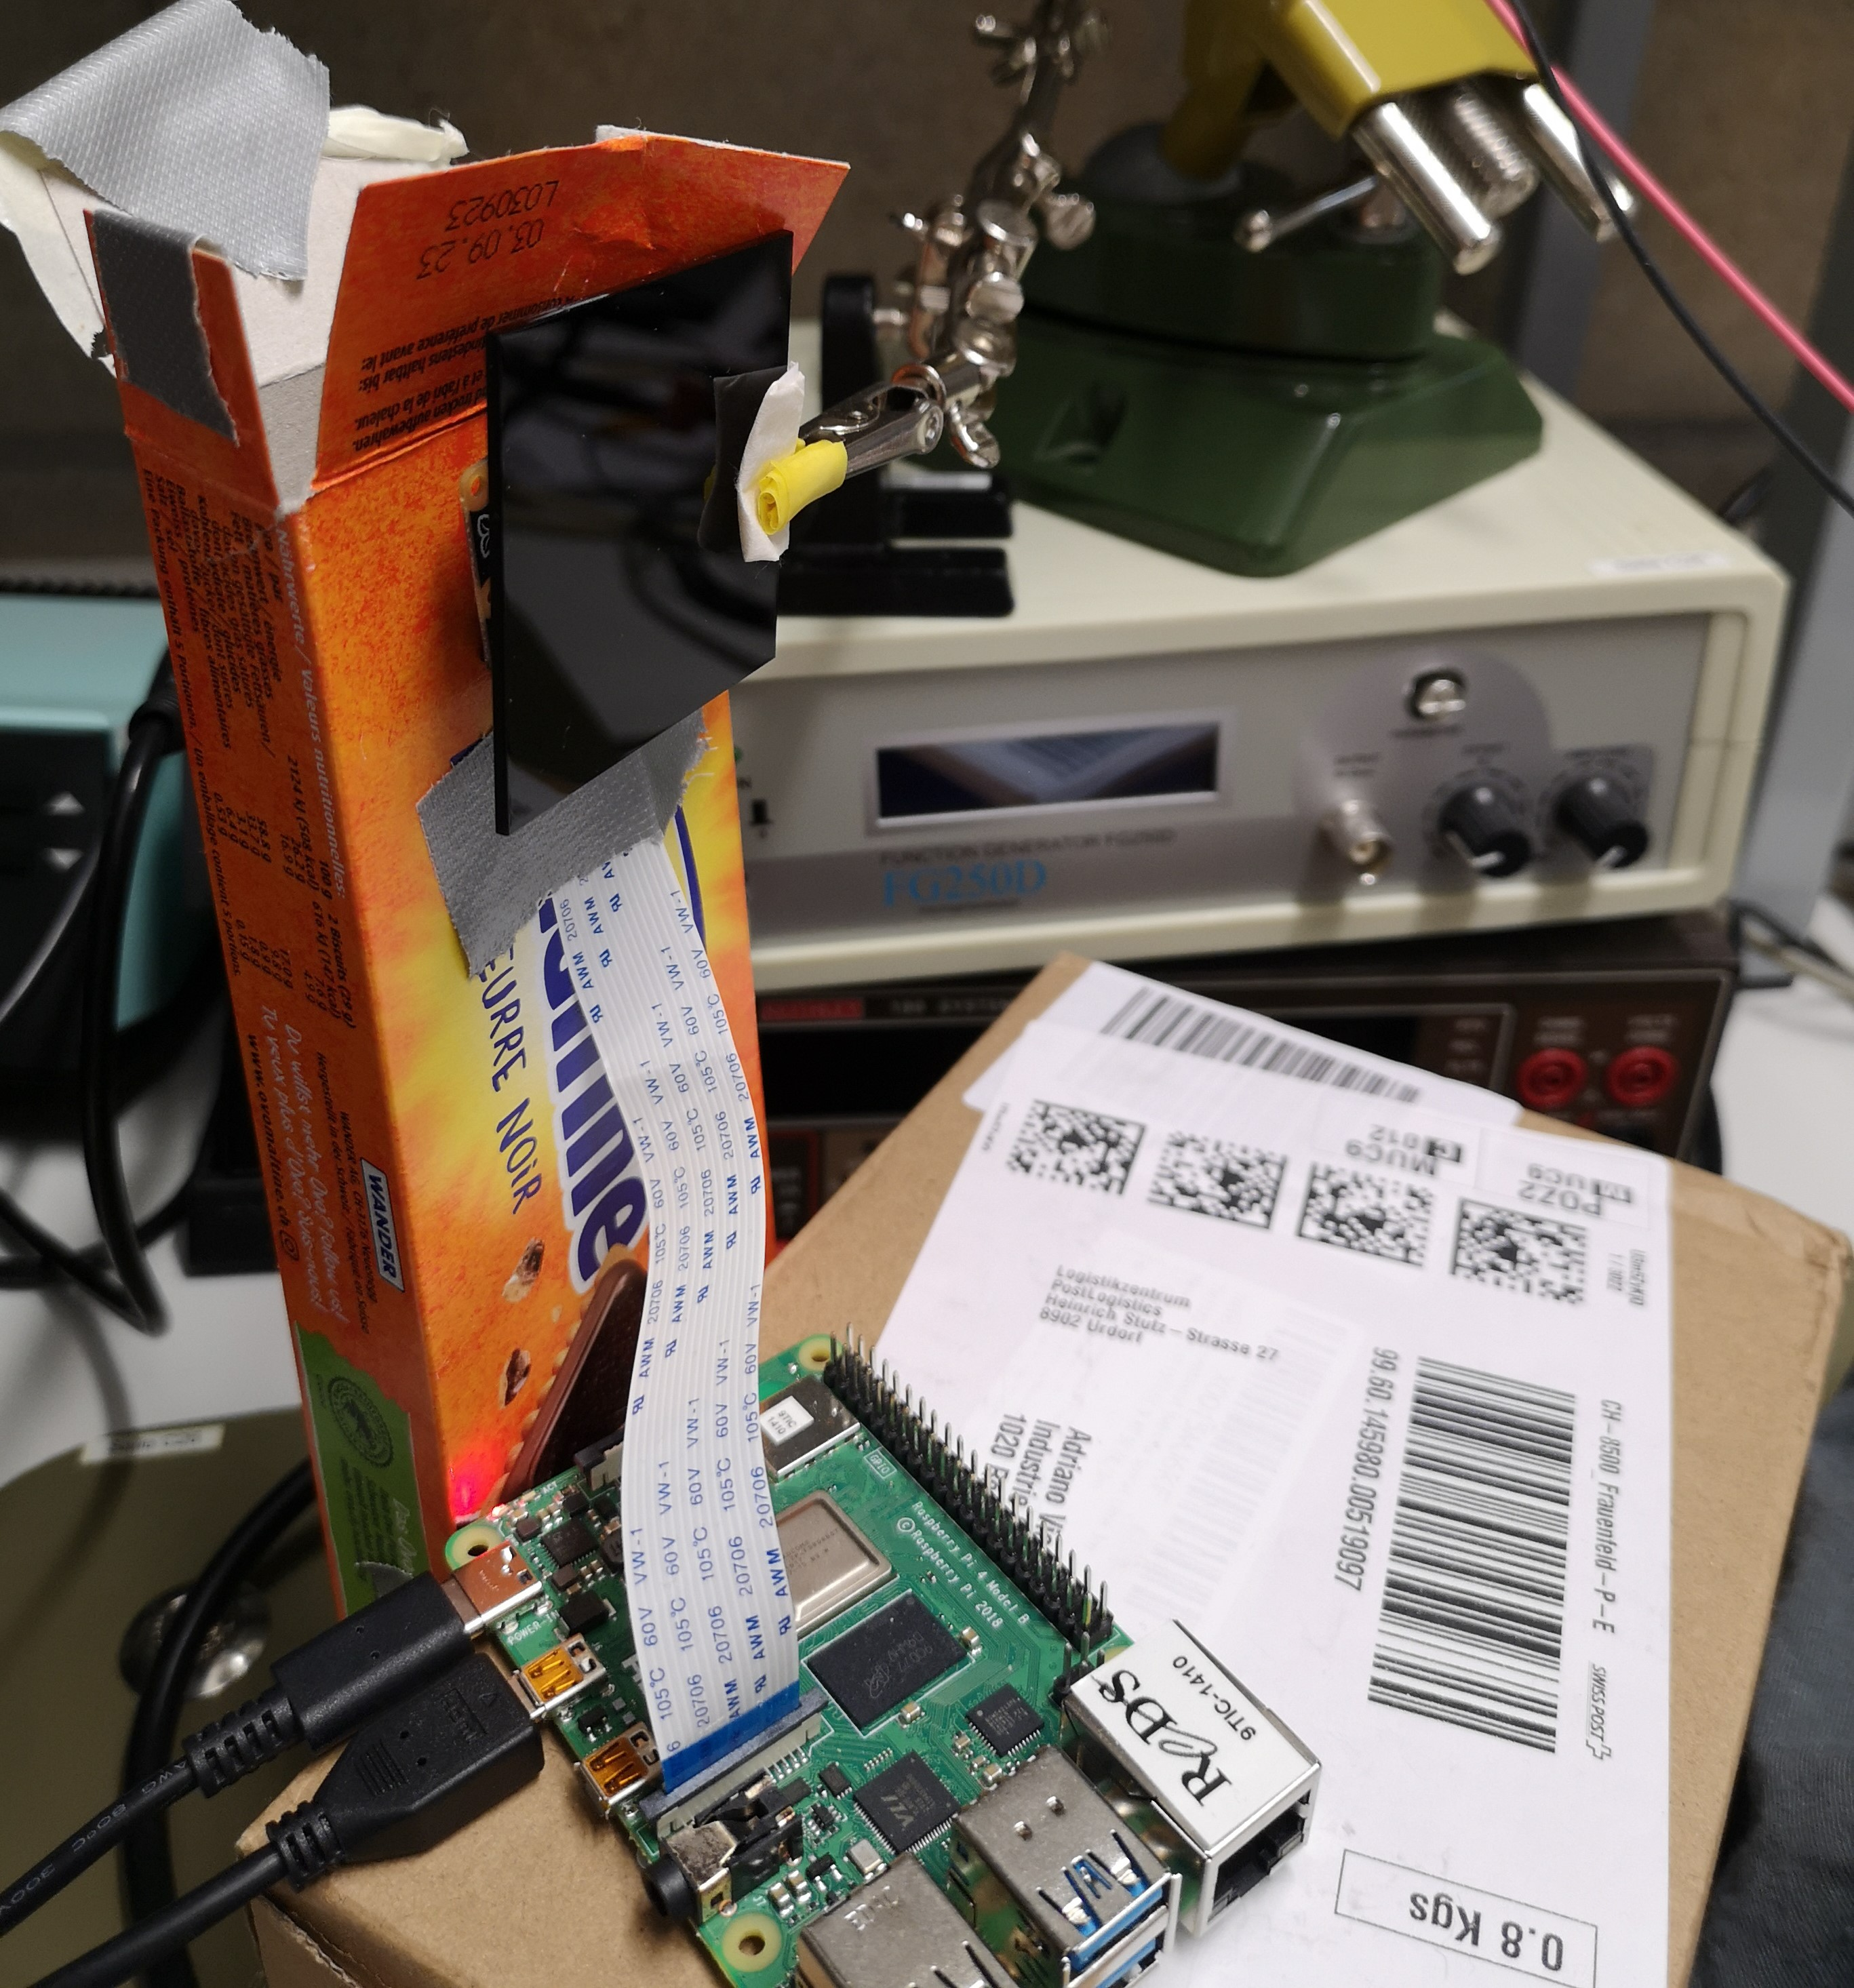
\includegraphics[height=13cm]{assets/figures/filtre.jpg}
    \caption{Capture avec filtre - Installation}
\end{figure}

Pour constater l'efficacité du filtre, j'ai effectué 3 captures.
\begin{itemize}
    \item Une image simple.
    \item Une image avec l'éclairage IR enclenché.
    \item Une image avec l'éclairage IR enclenché selon la figure \ref{led_perp}.
\end{itemize}
On notera également que le filtre perturbe l'autofocus du capteur, la position de la lentille a donc été définie en dur dans le code de test.
Les informations concernant ces réglages se trouvent au chapitre 5.2.3 de la documentation Picamera2 \cite{picamera2}.

\begin{figure}[H]
    \centering
    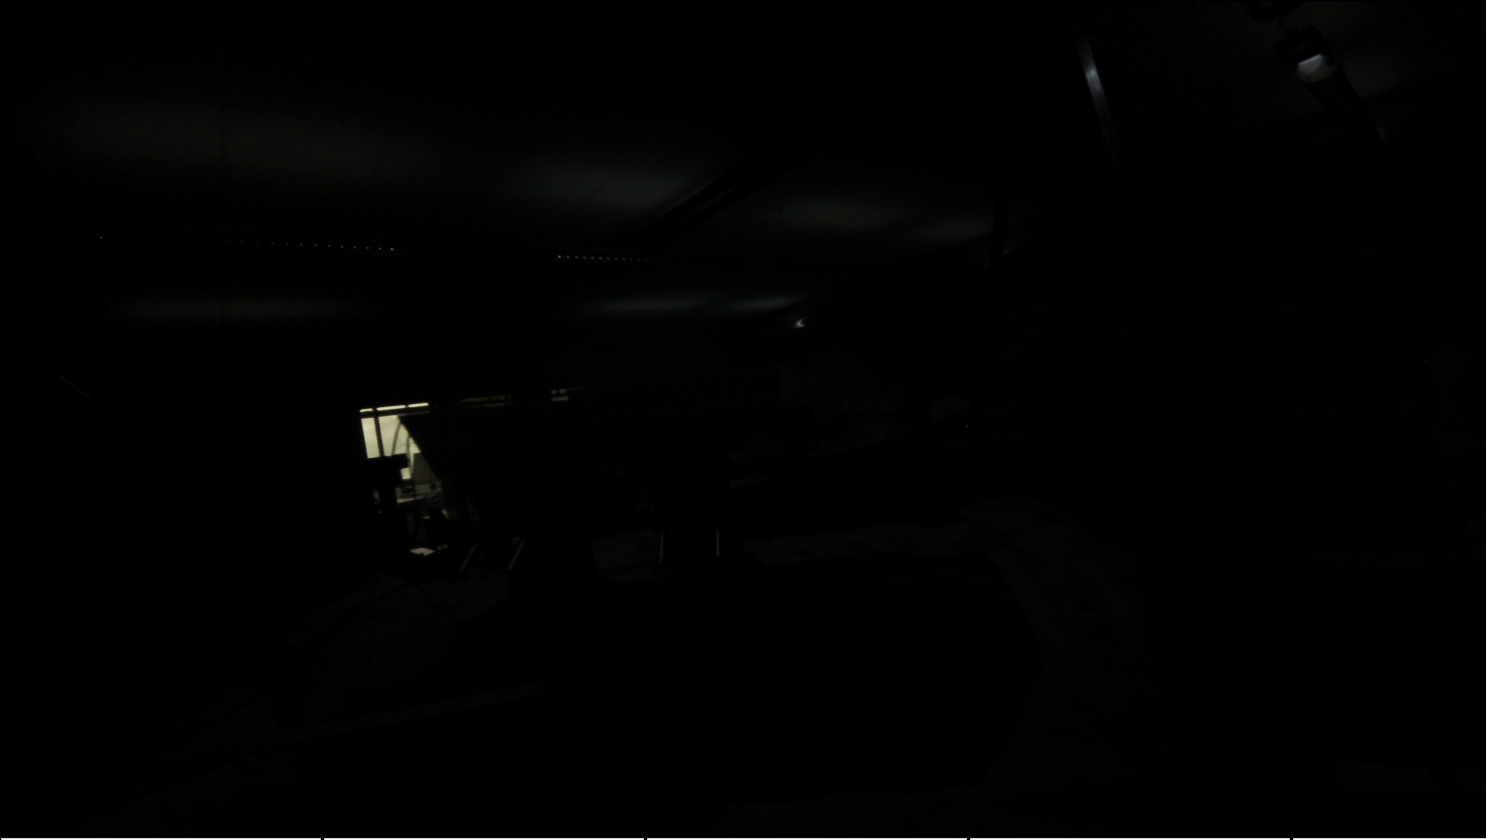
\includegraphics[width=13cm]{assets/figures/filtre_simple.png}
    \caption{Capture avec filtre - Environnement simple}
\end{figure}
\begin{figure}[H]
    \centering
    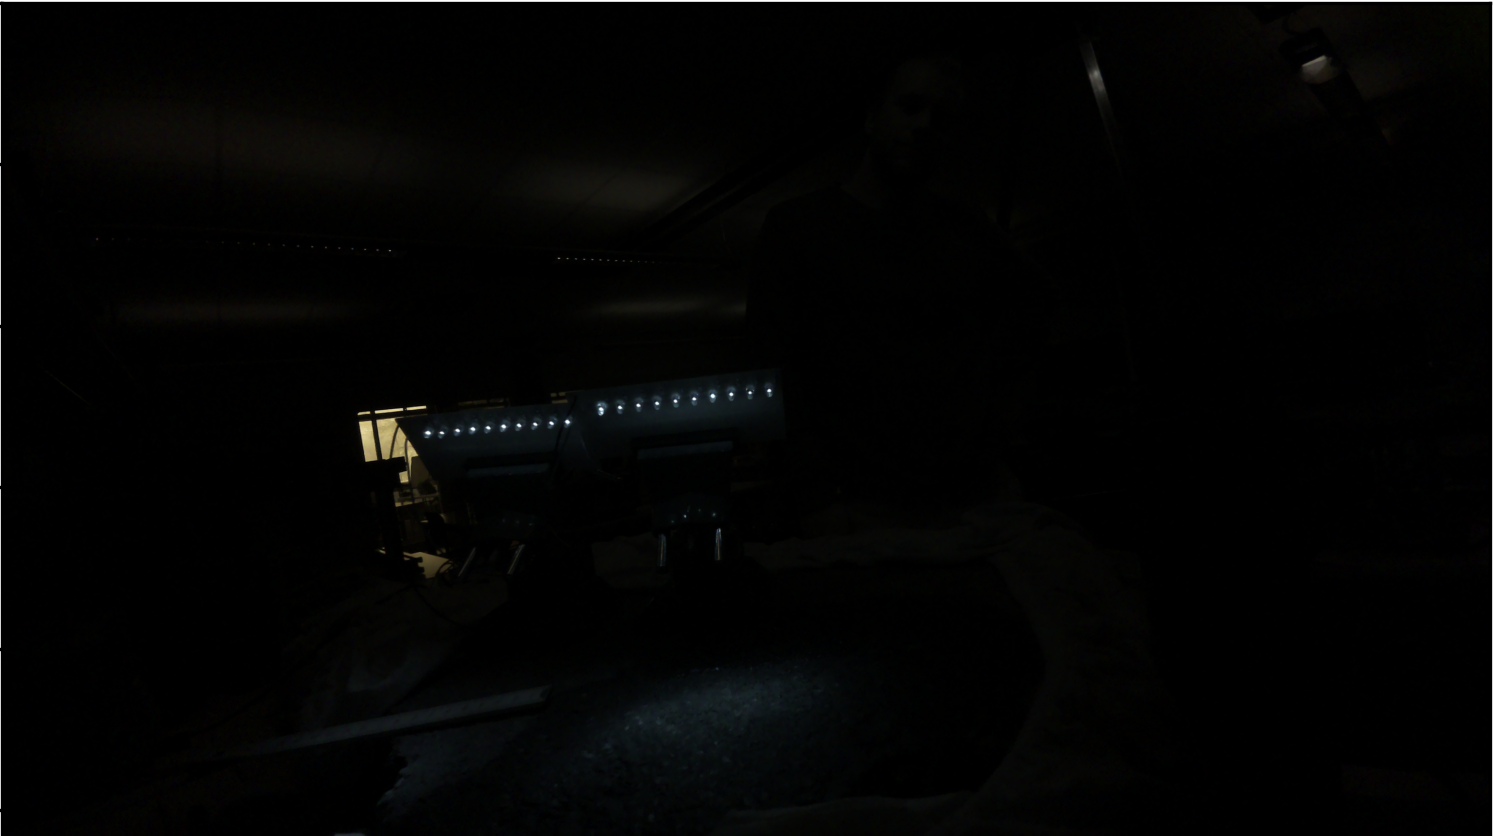
\includegraphics[width=13cm]{assets/figures/filtre_IR.png}
    \caption{Capture avec filtre - Leds IR allumées}
\end{figure}
\begin{figure}[H]
    \centering
    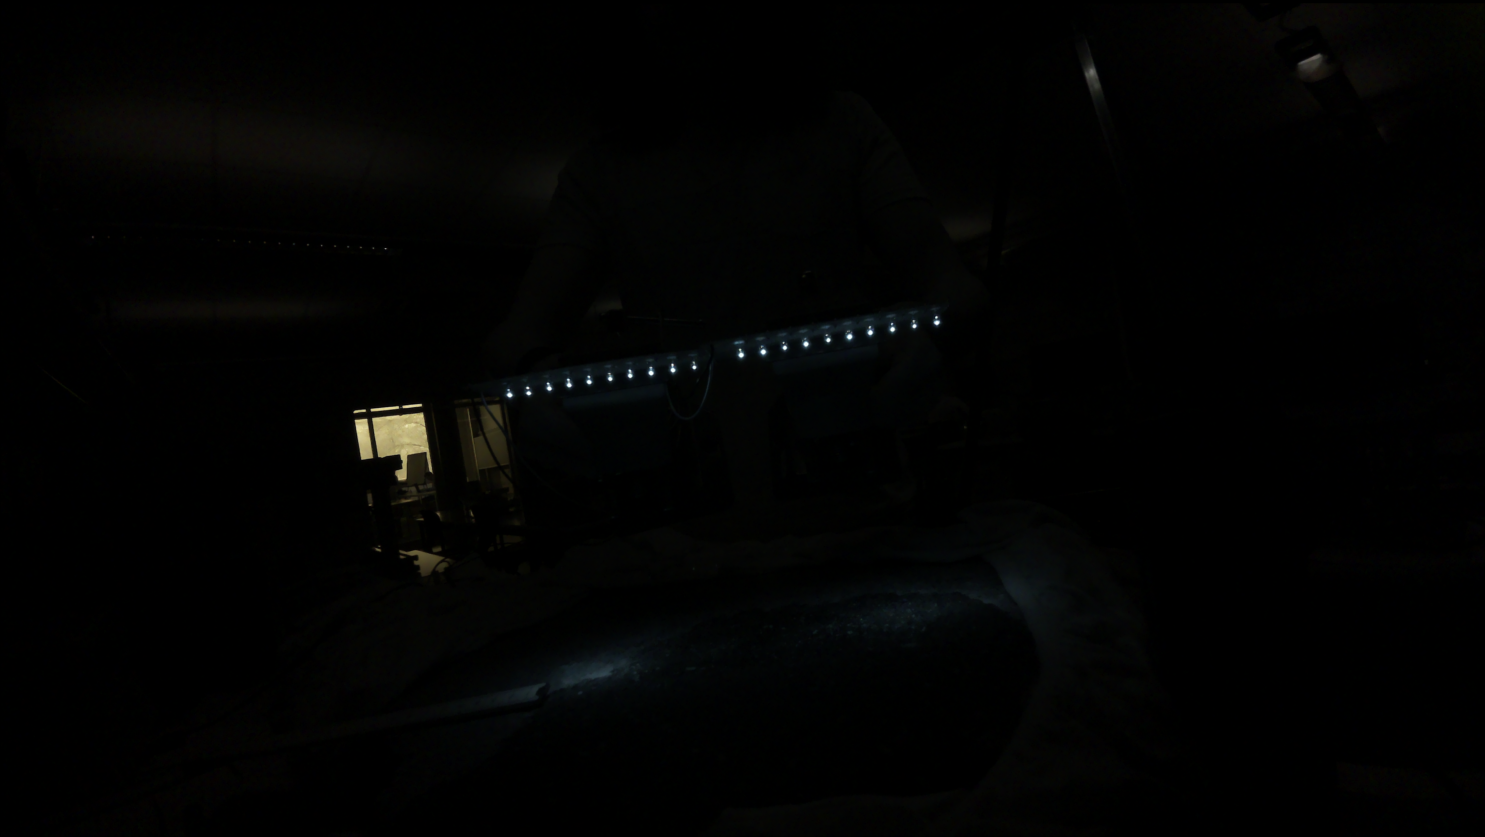
\includegraphics[width=13cm]{assets/figures/filtre_IR_huile.png}
    \caption{Capture avec filtre - Leds IR selon figure \ref{led_perp}}
\end{figure}
On observe que la quasi totalité des éclairages de la pièce disparaissent de la capture,
mettant en évidence la route et la trace d'huile au milieu de celle-ci. Il reste cependant les rayonnements solaires (visible sur la partie gauche des images)
à gérer, le soleil émettant dans un large spectre, ceux-ci apparaissent dans l'image. L'emplacement du laboratoire ne permet pas de
tester le filtre et le capteur sous un ensoleillement tel qu'on pourrait avoir en extérieur. De futurs tests sont nécessaires.

\section{Installation}
\subsection{Eclairage}
Le but est de garder le même principe d'éclairage que durant les tests préliminaires, c'est à dire une éclairage perpendiculaire au sol,
en bande, avec des leds IR émettant à 850nm. De plus, il faudrait que le système d'éclairage suive les contraintes suivantes:
\begin{itemize}
    \item Diffusion en bande.
    \item Largeur de 150cm.
    \item Repliable si non utilisés.
    \item Protégé pendant les déplacements.
\end{itemize}
J'envisage de faire fabriquer le rails de leds sur les principes suivants:
\begin{enumerate}
    \item Elément solide sur lequel braser les leds (veroboard).
    \item Structure solide sur lequel fixer les veroboards (rail).
    \item Elément de fixation permettant un repliage.
    \item Tube de protection à enfiler lors des transports.
\end{enumerate}
\subsubsection{Veroboard}
La plaque de veroboard sert de conducteur permettant aux leds d'être alimentées. L'objectif est d'avoir deux bandes de leds de 75cm de part et d'autre
du timon. Je n'ai pas trouvé de veroboard faisant cette largeur, j'ai donc décidé d'utiliser les plaques disponibles au FabLab de l'HEIG et d'en faire un assemblage.
Le but est de transformer 5 plaques de 6.6cm x 15cm en 10 plaques de 3.3cm x 15cm afin de couvrir la largeur requise avec un minimum d'épaisseur.
Chaque plaque serait reliée à la suivante via un connecteur afin de transmettre l'alimentation.

L'implantation sur veroboard se ferait selon le plan suivant:
\begin{figure}[H]
    \centering
    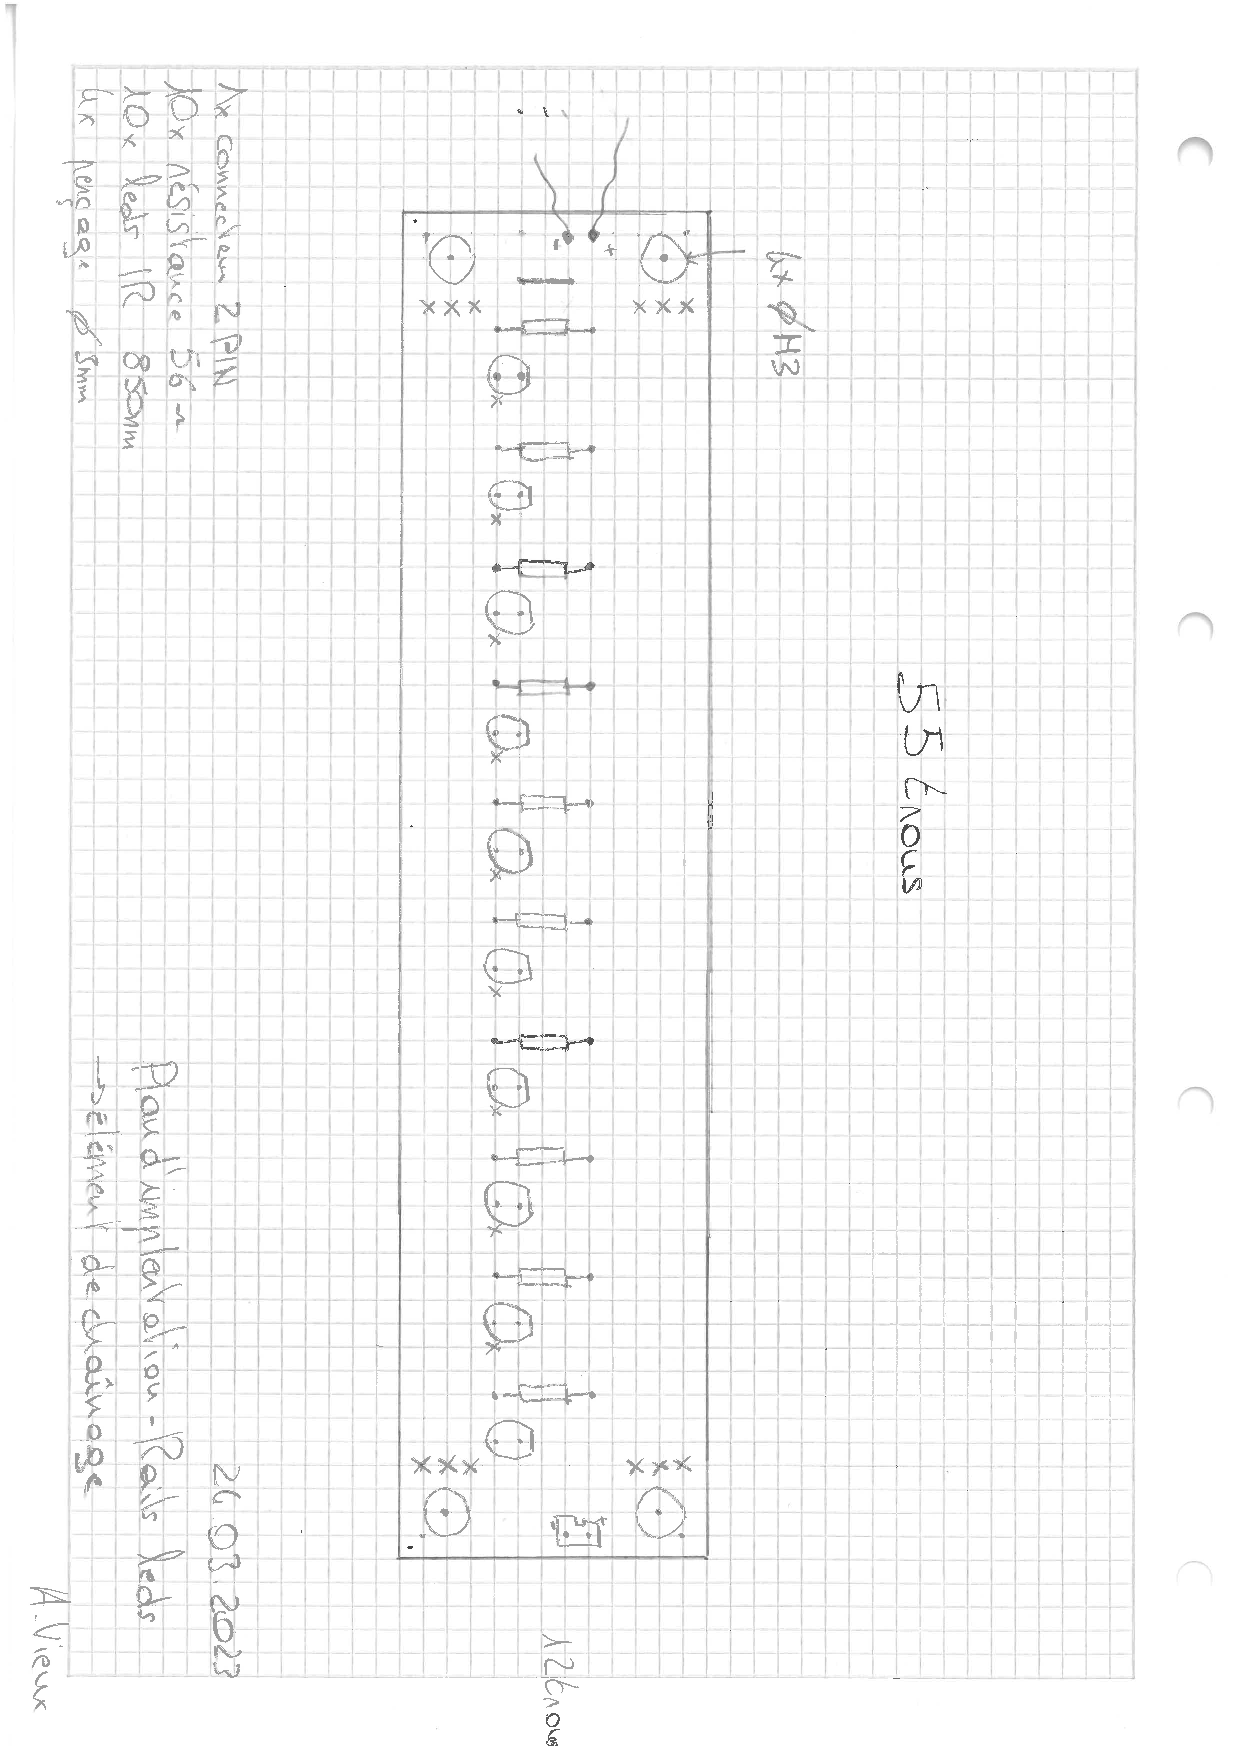
\includegraphics[width=13cm, trim=0 0 3cm 1cm, clip]{assets/figures/plan_implantation_rail_led.pdf}
    \caption{Plan d'implantation - Rail de Led}
\end{figure}

Notons que la chute de tension aux bornes des leds est de 1.3 V $\pm$ 0.1 V, celle-ci peut légèrement varier d'une led à l'autre. C'est
pourquoi il est important de mettre une résistance avant chaque led, de manière à ce que celle-ci gère le potentiel surplus de tension.
De plus, cela permet d'avoir un contrôle sur le courant traversant la led et donc sur l'intensité de l'éclairage. Durant les tests préliminaires,
le courant traversant les leds étaient de 3,5 \si{\milli\A}, l'intensité lumineuse était bonne, je décide donc de m'y tenir.

\begin{figure}[H]
    \centering
    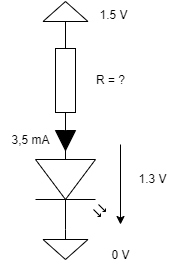
\includegraphics[height=7cm]{assets/figures/schema_led_res.png}
    \caption{Schéma électrique - Choix de résistance}
\end{figure}

Sachant \(R = U / I\), on se retrouve avec \(R = 0.2 / 0.0035 = 57.1 \si{\ohm} \) (Arrondi à 56\si{\ohm} dans la gamme de résistance E12).

\subsubsection{Rails}
Les veroboards ont été placés sur deux profilés plats en aluminium percées et équipées d'entretoises de manières à accueillir le tout. Il suffit de poser les veroboards,
les fixer à l'aide de rondelles et boulons et de relier les alimentations d'une carte à l'autre. En cas de panne, le remplacement de la carte problématique est très rapide.

\begin{figure}[H]
    \centering
    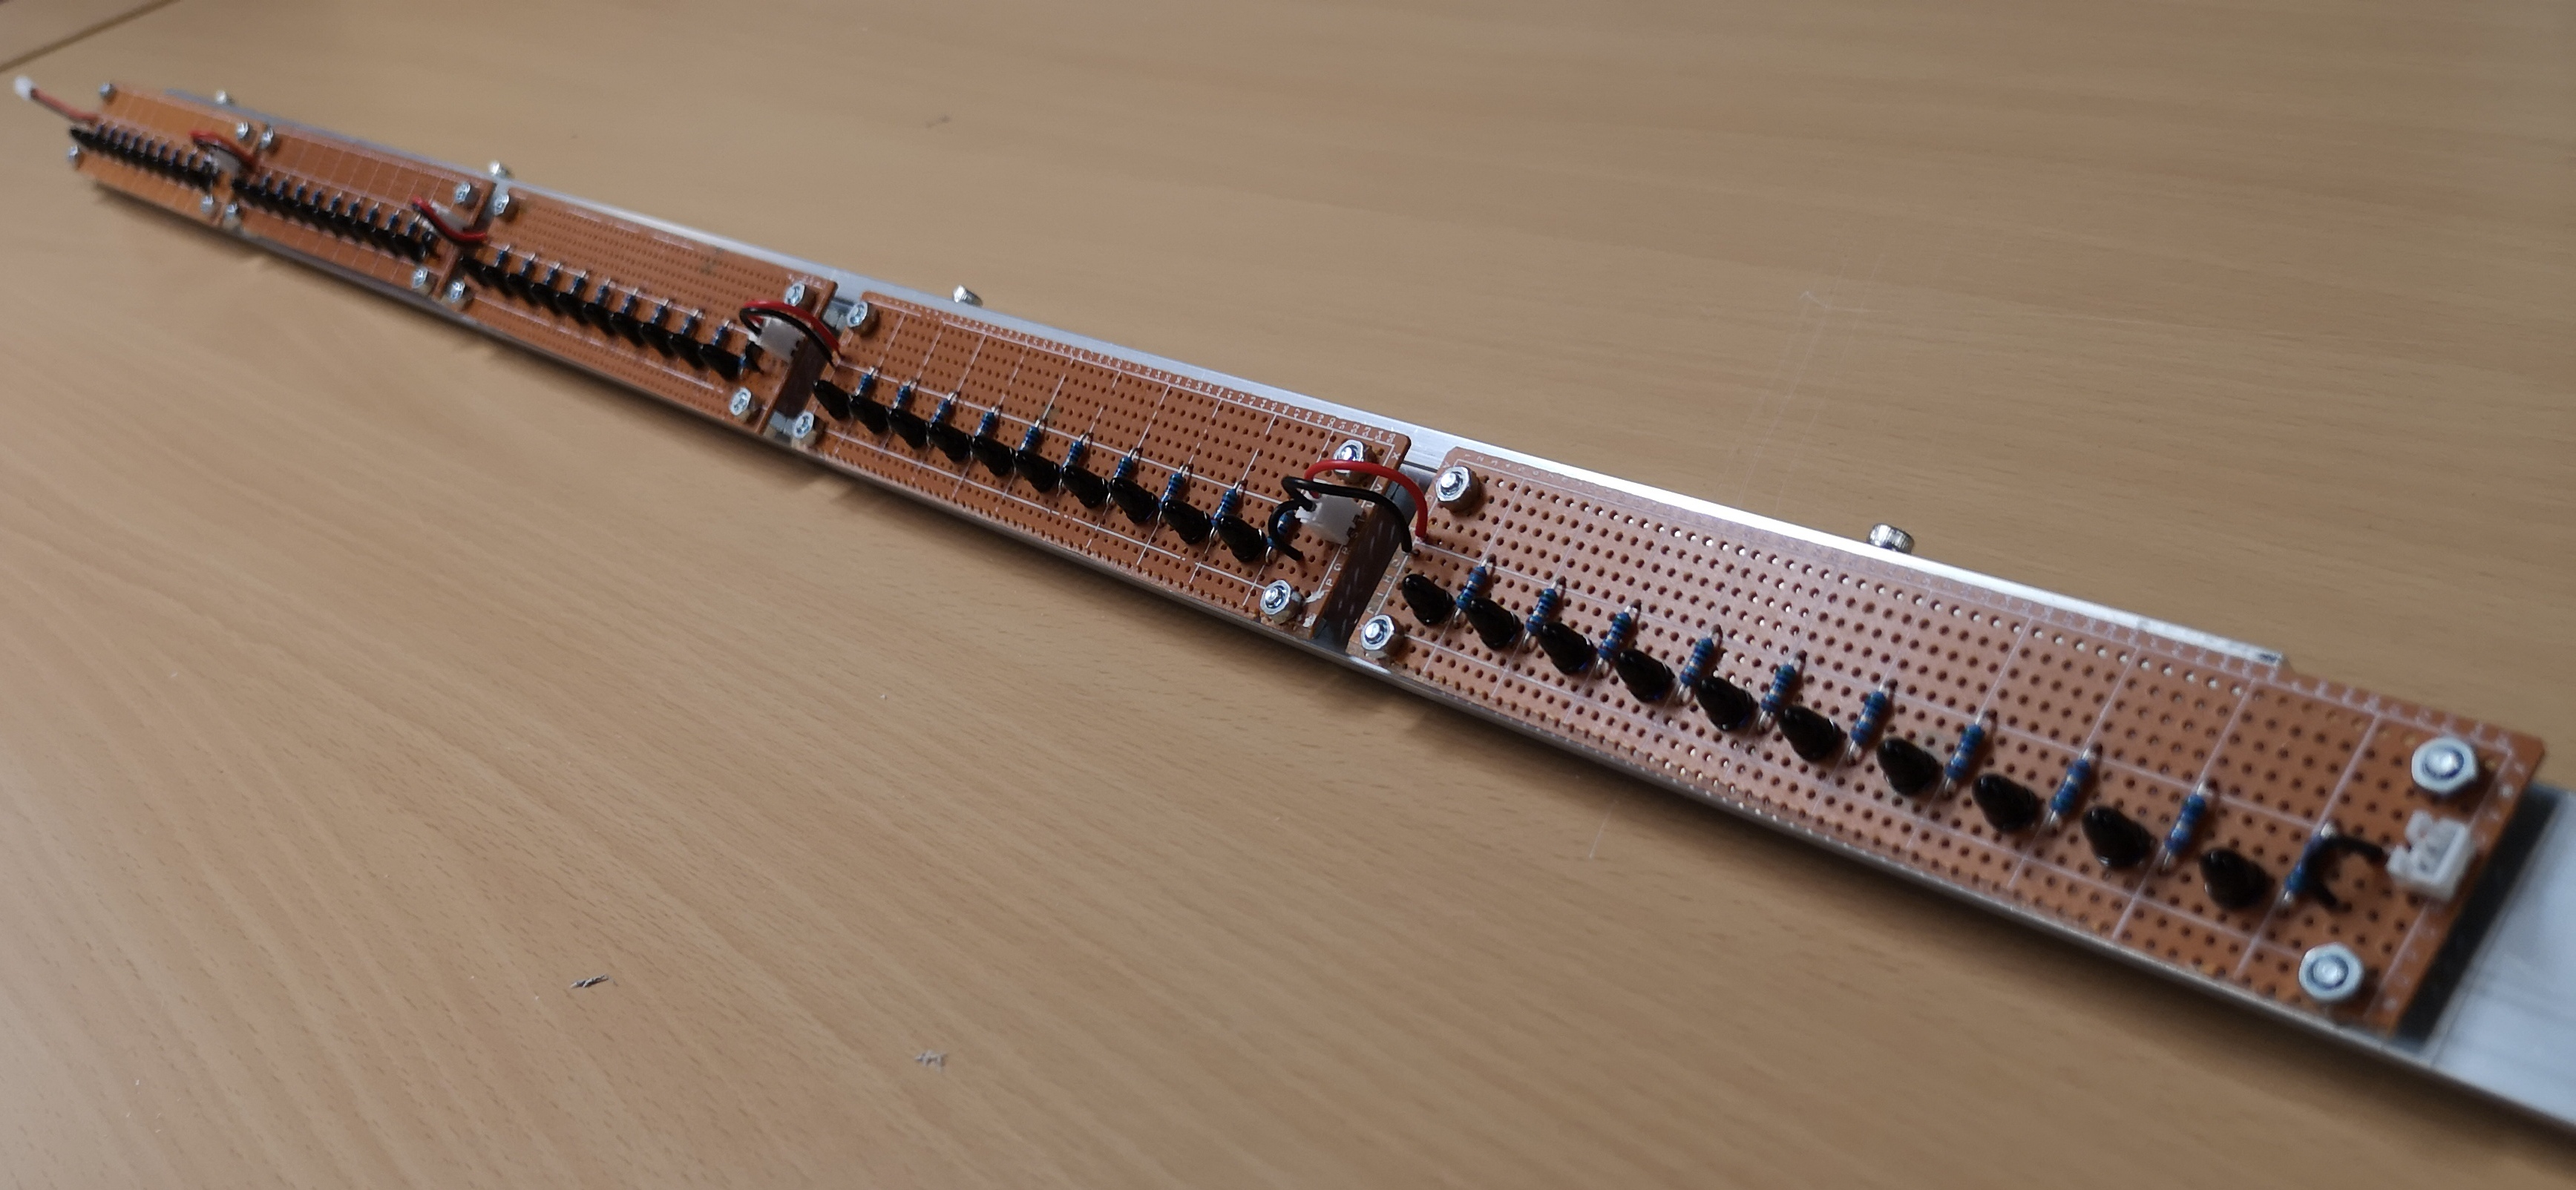
\includegraphics[height=7cm]{assets/figures/rail_alu_led.jpg}
    \caption{Assemblage - Rail led sur profilé plat}
\end{figure}

On notera qu'un second élément en aluminium a été vissé perpendiculairement au premier de manière à limiter les vibrations sur le rail d'éclairage.

\subsection{Caméra}
Dans le but d'avoir la caméra le plus centré possible, la caméra ...
\section{Programme}
\subsection{Librairies}
indiquer les pip install à faire et toute les lignes pour préformater le rpi4
\subsection{Capture d'images de références}
\subsubsection{Paramètres}
Le traitement d'image permettant de mettre en valeur et détecter les hydrocarbures nécessite des images de références ayant été capturées dans des conditions précises et avec des paramètres de caméra maîtrisée.

Le programme de capture d'image de références fera plusieurs centaines de capture de la même zone à observer en faisant varier les paramètres suivants:
\begin{itemize}
    \item Temps d'exposition
    \item Gain analogique
    \item Balance des blancs
\end{itemize}

Le programme \underline{cap\_img\_ref.py} (annexe [faire ref]) effectue les changements de paramètres et capture 3 images par configuration.

(D'après la documentation de la caméra, l'ajustement des paramètres s'effectue en 3 frames maximum.)
Au terme des essais, la configuration idéal est la suivante:

\begin{table}[H]
    \begin{center}
        \caption{Table - Configuration caméra}
        \begin{tabular}{|c|c|}
            Elément              & Valeurs                \\ \hline
            Temps d'exposition   & 500 \si{\milli\second} \\
            Gain analogique      & 4.0                    \\
            Balance des blancs R & 0.7                    \\
            Balance des blancs B & 1.5                    \\
        \end{tabular}
    \end{center}
\end{table}

Cet configuration permet de..
\subsubsection{Résultats}
Une première séance de capture directement m'a permis d'effectuer des captures à l'aide du code mentionné précédemment: \underline{cap\_img\_ref.py}. Cependant, j'ai rencontré un problème, les captures sont floues, laissant penser que la mise au point est mal réglée.

METTRE UNE OU DEUX IMAGE DE LA SEANCE

La librairie Picamera2 \cite{picamera2} comprend une méthode qui règle la position de la lentille en fonction de la distance souhaitée pour la mise au point. La méthode a été testée en laboratoire et fonctionnait très bien. Durant la séance de capture,
la mise au point était définie pour observer les éléments à 90 \si{\centi\meter} de l'objectif.

En reproduisant le problème en laboratoire, j'ai compris que c'est la vitre de protection qui pose problème, en la retirant ou simplement en mettant de la distance entre la vitre et l'objectif, l'image redevient nette.

J'estime donc qu'il y a plusieurs solutions qui s'offrent à moi.
\begin{enumerate}
    \item Jouer avec le paramètre du focus et trouver une valeur pour laquelle on a une image nette derrière la vitre.
    \item Revoir le placement de la caméra dans le boitier de manière à ne pas coller l'objectif à la vitre.
    \item
\end{enumerate}

\subsection{Traitement de l'image}
\subsubsection{Structure du programme}
UML ou séquence de traitement
\subsubsection{Astuce de codage}
Code ou morceau de code clé -> lien vers les annexes
\subsection{Communication}

\chapter{Contrôle de la télécommande}
\section{Tests préliminaires}
Le but des tests préliminaires est de vérifier que les analyses effectuées dans la phase de recherche sont applicables et si la mise en
place du système imaginé lors de la phase de sélection du matériel est aussi efficace qu'espéré.

Il a été décidé de contrôler la télécommande via un système de préhenseur d'aimant de levage. Les données disponibles de la télécommande
ne stipule pas la force nécessaire à l'activation d'un de ses boutons, plusieurs préhenseurs sélectionné dans le stock du \Gls{fablab}
sont utilisés pour définir la force nécessaire à l'activation des touches.

\begin{itemize}
    \item Préhenseur 6VDC 4W, 0.4N -> 2N.
    \item Préhenseur 12VDC 7W, 0.6N -> 11N.
\end{itemize}

Les préhenseurs ont été installés sur une pièce imprimée en 3D permettant d'actionner la télécommande sans avoir des effets de reculs.
La hauteur est determinée de manière à pouvoir glisser la télécommande entre les plauqes tout en garantissant que la tige puisse se déployer sur
une longueur suffisante pour atteindre son pic de force.

\begin{figure}[H]
    \centering
    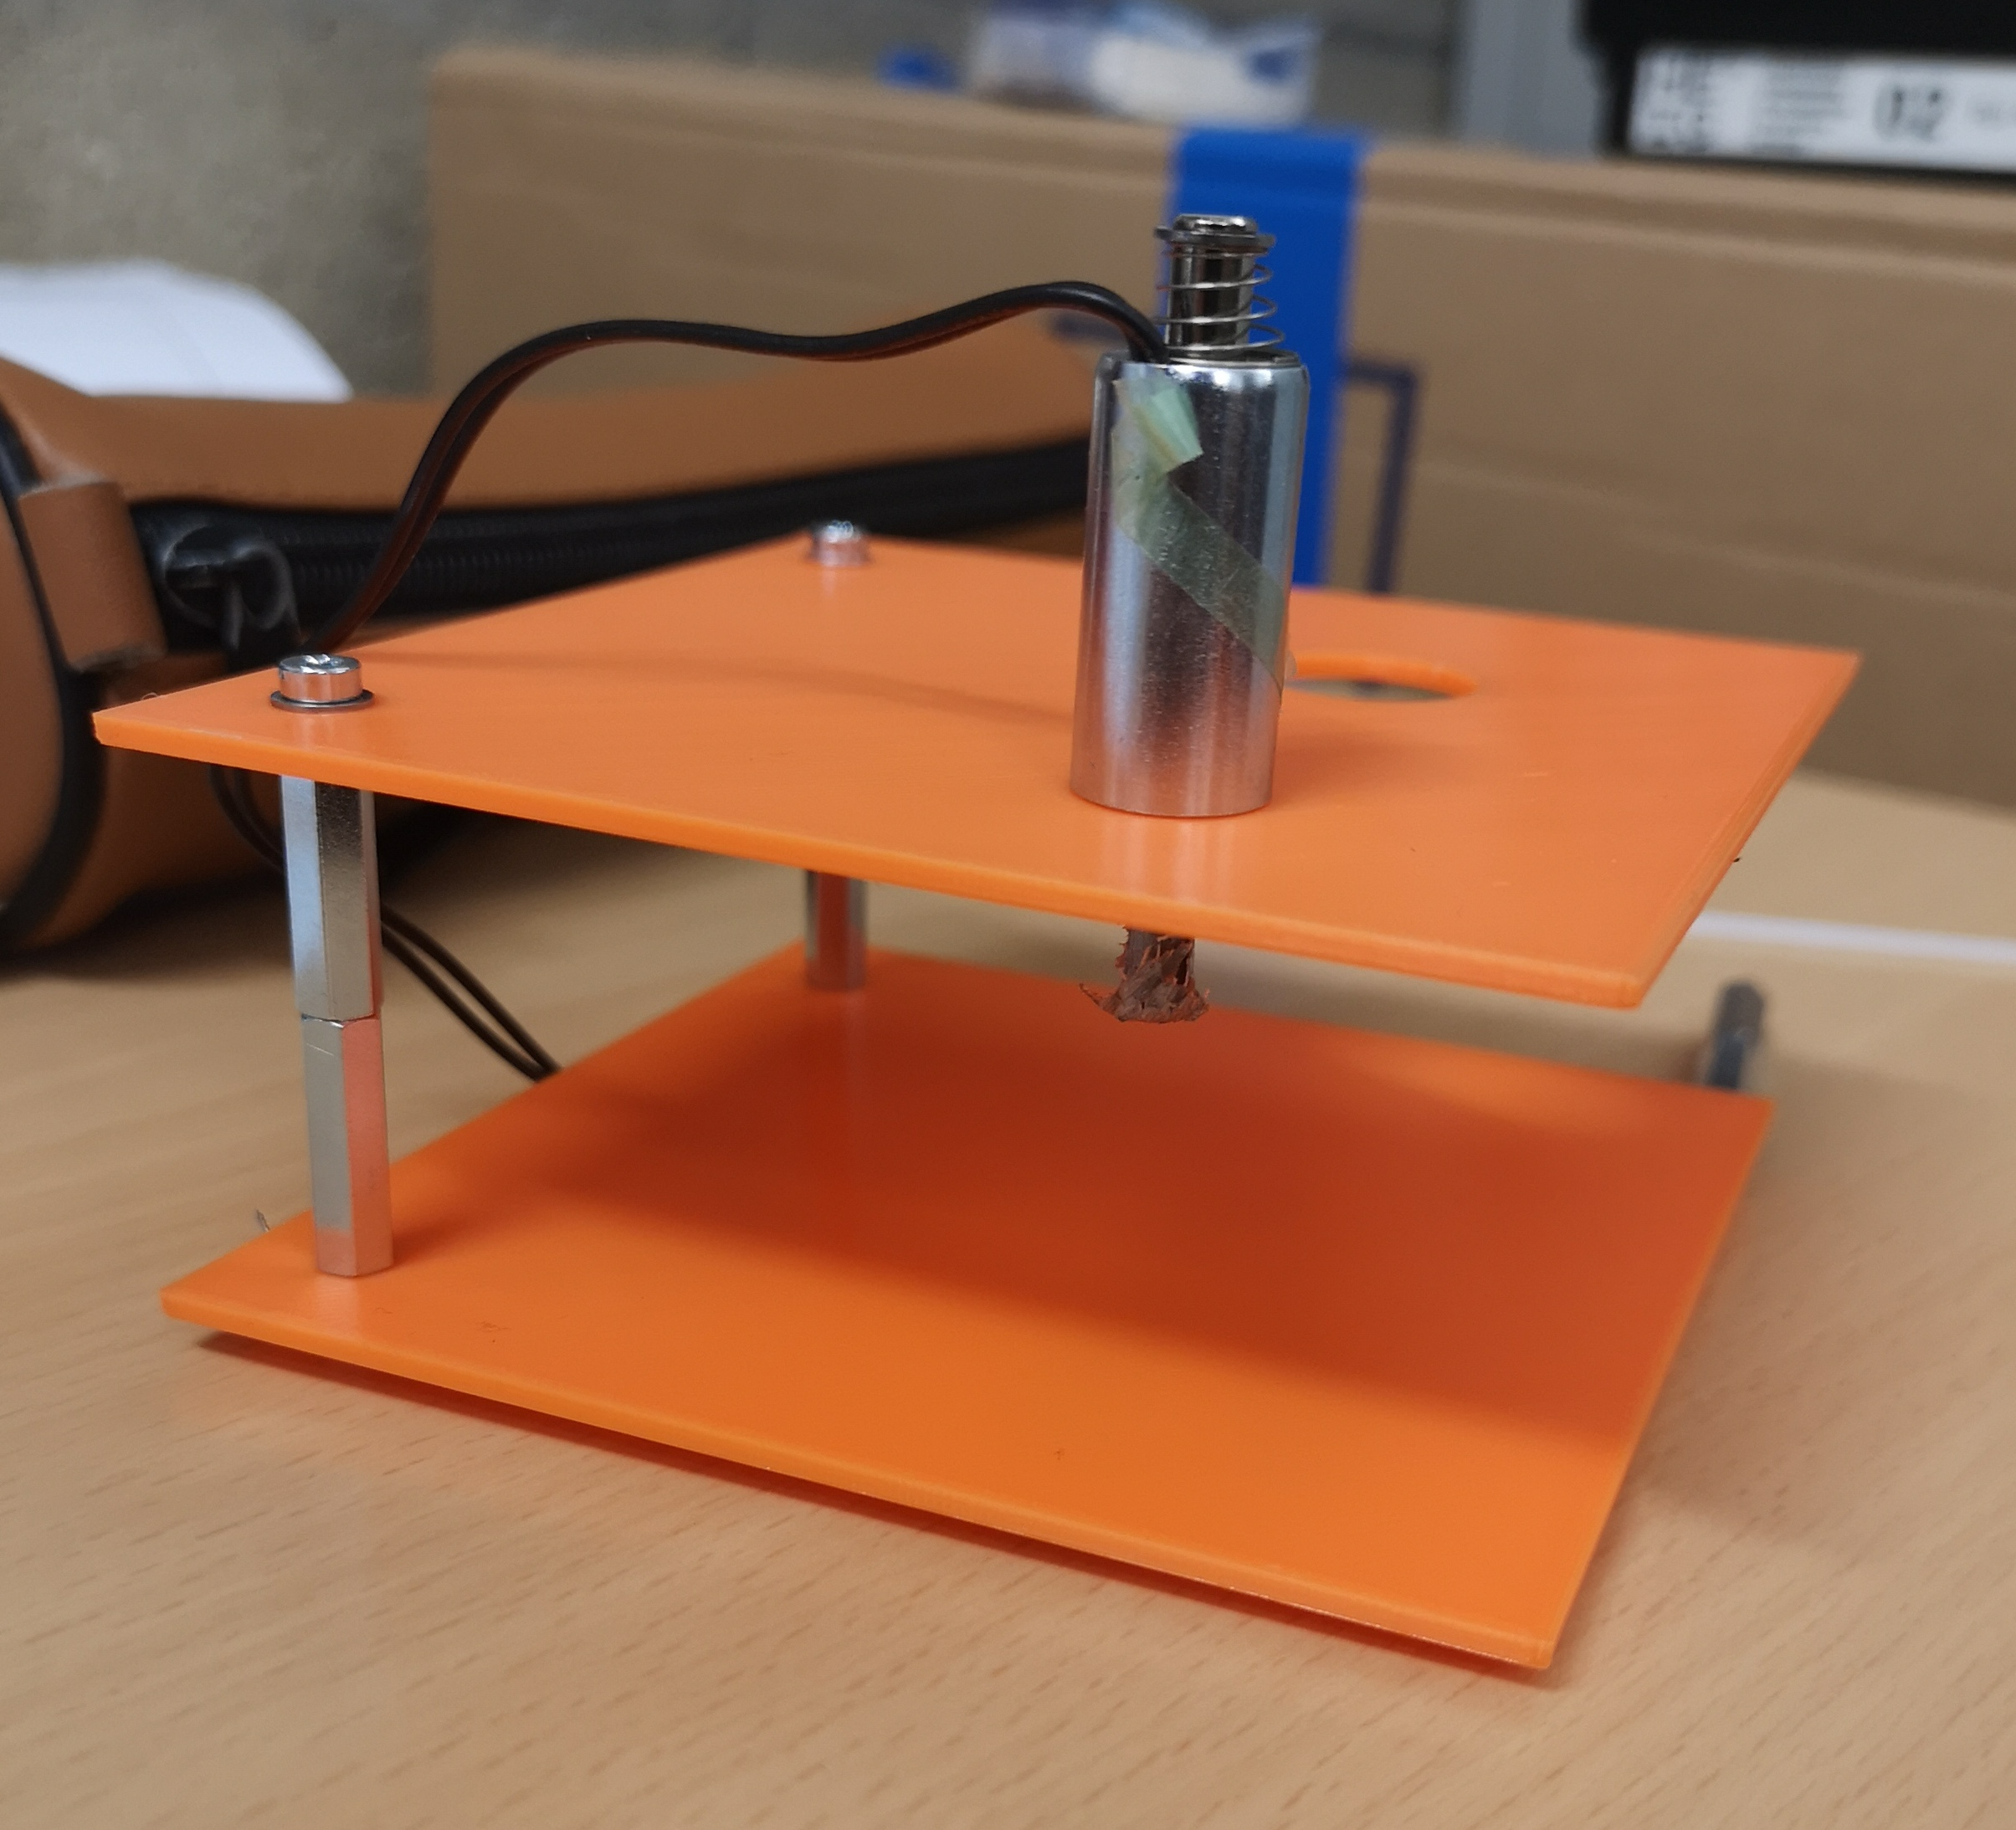
\includegraphics[width=10cm]{assets/figures/support_test_prehenseur.jpg}
    \caption{Système de préhension - Support de test}
\end{figure}

\begin{table}[h]
    \begin{center}
        \caption{Résultats du test de préhension}
        \begin{tabular}{|c|l|}
            Elements       & Boutons \\ \hline
            Préhenseur 2N  & OUI-NON \\
            Préhenseur 11N & OUI-NON \\
        \end{tabular}
    \end{center}
\end{table}\\

\section{Supports}

\subsection{Support pour jeu de préhenseur magnétique}
\subsection{Support de la télécommande}

\section{Programme}
\subsection{Pilotage des vérins}
\subsection{Communication}

\chapter{Retour vidéo}
\section{Communication}
Il a été décidé durant la phase de recherche que l'affichage se fera via un écran "volant" qui recevera les images via un réseau WiFi local
hébergé par le Rapsberry Pi. Les étapes pour y arriver sont les suivantes:
\begin{enumerate}
    \item Flasher avec l'OS Rapsberry (en utilisant Rapsberry imager ou BalenaCloud).
    \item Être connecté à internet.
    \item Télécharger le package 'dnsmasq': \textbf{sudo apt-get install dnsmasq}.
    \item Atteindre le fichier suivant: \textbf{sudo nano /etc/wpa\char`_supplicant/wpa\char`_supplicant.conf}.
    \item Y ajouter le code du listing \ref{wpa}, sauver + quitter: ctrl+O, puis ctrl+X.
    \item Atteindre le fichier suivant: \textbf{sudo nano /etc/network/interfaces}.
    \item Y remplacer le code du listing \ref{interfaces}, sauver + quitter: ctrl+O, puis ctrl+X.
    \item Atteindre le fichier suivant: \textbf{sudo nano /etc/dnsmasq.conf}.
    \item Y remplacer le code du listing \ref{dnsmasq}, sauver + quitter: ctrl+O, puis ctrl+X.
    \item Redémarrer le Rpi4 avec: \textbf{sudo reboot}.
    \item Couper la connexion réseau avec: \textbf{sudo ifdown wlan0}.
    \item Accéder à la liste des réseaux avec: \textbf{sudo wpa\char`_cli -i wlan0 list\char`_networks}, puis saisir le réseau avec: \textbf{sudo wpa\char`_cli -i wlan0 select\char`_network 1} (exemple figure..)
    \item Sauver la nouvelle configuration avec \textbf{sudo wpa\char`_cli -i wlan0 save\char`_config}.
    \item Relancer la connexion réseau avec: \textbf{sudo ifup \underline{wlan0=ap0}}.
\end{enumerate}
\begin{listing}[ht]
    \inputminted{makefile}{assets/figures/wpa_supplicant.make}
    \caption{Configuration wpa\char`_supplicant \label{wpa}}
\end{listing}

\begin{listing}[ht]
    \inputminted{makefile}{interfaces.make}
    \caption{Configuration de l'interface réseau \label{interfaces}}
\end{listing}

\begin{listing}[ht]
    \inputminted{makefile}{dnsmasq.make}
    \caption{Configuration dnsmasq \label{dnsmasq}}
\end{listing}

Avec l'ajout de ces lignes, le Rpi4 emet un réseau local dès son démarrage. Il est possible de s'y connecter avec n'importe quel
type d'appareil. Le nom du réseau et le mot de passe sont paramétrables, actuellement, c'est:
\begin{itemize}
    \item Nom du réseau: \textbf{SemoirSDIS}
    \item Mot de passe: \textbf{123456789}
\end{itemize}\\
À noter qu'il est obligatoire de s'y connecter pour avoir le retour vidéo.

\begin{figure}[H]
    \centering
    
\includegraphics[width=3cm]{assets/figures/acces_wifi.PNG}
    \caption{QR code - Connexion WiFi local}
\end{figure}

\section{Affichage}
Il existe des codes sources disponibles en ligne permettant d'afficher le retour caméra basé sur le package Picamera2 \cite{picamera2}.
Je me suis inspiré de celui-ci pour mon affichage: \cite{code_camera}.\\
L'utilisation de \textbf{Picamera2} nécessite l'installation de dépendances:
\begin{itemize}
    \item \textbf{sudo apt-get install libatlas-base-dev}.
\end{itemize}
\textbf{Mettre screenshot du rendu sur natel/pc}\\
Mettre le code source en annexe.
\section{Accès}
L'accès au retour vidéo se fait via une page locale dont l'accès nécessite d'être connecté au WiFi émis par le Rpi4.
La page se trouve à l'adresse statique suivante:
\begin{itemize}
    \item  \url{192.168.0.1:8000/index.html}
\end{itemize}
Accès rapide:

\begin{figure}[H]
    \centering
    
\includegraphics[width=3cm]{assets/figures/acces_stream.PNG}
    \caption{QR code - Connexion stream}
\end{figure}

\chapter{Conclusion}
\section{planning}
METTRE SCREEN ET COMMENTER

\section{Ressenti personnel}
La ou en temps normal il y une semaine entre deux jours de travail permettant de réfléchir, là y'a rien, très vite frustrant si bloqué plus de quelques heures..

Gardé mon calme et avancé comme je pouvais, fréquence d'entre vue plus élevée permettait de rester sur les rails.

Edition du rapport en latex chaud pour une première

Donner ressenti en fonction de l'état du proto
\section{Conclusion technique}
Difficulté projection aspect mécanique
Condition de test très différent de condition extérieur, ne pas savoir avec exactitude ce qu'on verra

Concilier avance rapide et choix de composants

Découverte de l'électronique embarquée et de mécanique, pas super propre, mais prototype plus ou moins fonctionnel.

Donner l'état du proto en fin de projet fonctionnel ou pas tout à fait

Parler du planning, parler des différences, résultat en annexe.
\section{Remerciement}
Je tenais à remercier les différentes personnes qui m'ont entourés, accompagnés et aidés durant ce projet.

Je remercie M. Tristan Lieberherr, qui m'a partagé ses connaissances sur les Raspberry Pi et sur la configuration des réseaux WiFi locaux.

Je remercie M. Nicolas Tzaut, qui m'a très gentiment céder un morceau de route provenant de sa démolition, grâce auquel j'ai pu effectué
des tests de capture d'image en laboratoire très rapidement après le début du projet.

Et je remercie finalement M. Pierre Bressy, qui m'a suivi tout du long du projet. Il a su me... et me donner de nouvelles idées lorsque
j'étais bloqué.
\vfil
\hspace{8cm}\makeatletter\@author\makeatother\par
\hspace{8cm}\begin{minipage}{5cm}
    %%if
    % Place pour signature numérique
    \printsignature
    %%fi
\end{minipage}

\clearpage
\printbibliography

\appendix
\appendixpage
\addappheadtotoc

%%if
\chapter{Première annexe}

Les annexes n'ont pas un contenu \underline{normatif} mais \underline{descriptif}. Tout contenu annexé ne doit pas être nécessaire à la bonne compréhension du travail.

Les annexes contiennent généralement :

\begin{itemize}
    \item les dessins mécaniques (mises en plan);
    \item les schémas électriques détaillés;
    \item des photographies du projet;
    \item des scripts et des extraits de code source;
    \item des documents techniques \pex \emph{datasheet};
    \item des développements mathématiques.
\end{itemize}
\section{Sous section}
\lipsum[1]
%%fi

\let\cleardoublepage\clearpage
\backmatter

\label{glossaire}
\printnoidxglossary
\label{index}
\printindex

% Le colophon est le dernier élément d'un document qui contient des notes de l'auteur concernant la mise en page et l'édition du document : il est parfaitement optionnel.
\input{colophon.tex}

\end{document}
